%	Next lines is for compiling with arara package

%	First compiling: useful for generating .sxd files of the index
%	arara: pdflatex

%	Generate .sbx files of the index
%	arara: songidx: {input: ./chiesa}
%	arara: songidx: {input: ./party}
%	arara: songidx: {input: ./christmas}

%	Last compiling with complete indexes
%	arara: pdflatex


\documentclass[openright]{book}
%	Preamble
\usepackage[a5paper,left=15mm,right=15mm,bottom=10mm,top=15mm]{geometry}
\usepackage[utf8]{inputenc} % For special sybols
\usepackage{graphicx} % For pictures
\usepackage{latexsym} % For arrow
\usepackage{ulem} % For \xout
\usepackage{ifthen} % For if-then-else funtions
\usepackage[bookmarks]{hyperref} % For indexes

%\usepackage[italian]{babel} % For italian language

%	Header and footer
\usepackage{fancyhdr}
	\pagestyle{fancy}
%	\renewcommand{\chaptermark}[1]{\markboth{\textsc{#1}}{}}
	\fancyhf{}
	\fancyhead[LE,RO]{%\thepage
	}
	\fancyhead[RE,LO]{%\leftmark
	}
  \fancyhead[C]{%\leftmark
  }

%	\fancyfoot[C]{
\includegraphics[]{img/cc-by-sa_80x15.png}}

	\renewcommand{\headrulewidth}{0pt}
	\renewcommand{\footrulewidth}{0pt}

%	Songs package and its parameters
\usepackage[chorded]{songs} % For chords book (xor with lyric)
%\usepackage[lyric]{songs} % For lyrics book (xor with chorded)
	\nosongnumbers
	%\noversenumbers
	%\includeonlysongs{37,50,2}
	\prefersharps % For automatic transpositions

%	Indexes
	\newindex{chiesa}{chiesa}
	\newindex{party}{party}
	\newindex{christmas}{christmas}

%	Fonts
	\renewcommand{\lyricfont}{\sffamily}
	\renewcommand{\printchord}[1]{\rmfamily\bf#1}

	\songcolumns{1} % Number of columns for every page

%	Page-breanking and column-breaking
	\spenalty=-10000	% At song boundaries (-10000: the break is required)
%	\brkpenalty=200		% Wherever \brk is used
%	\vvpenalty=50 		% Verse to verse breaking
%	\ccpenalty=50 		% Chorus to chorus breaking
%	\vcpenalty=50 		% Verse to chorus breaking
%	\cvpenalty=50 		% Chorus to Verse breaking

  \songpos{3} % Aggressiveness of song-positioning algorithm

%	The width of the shaded boxes that begin each alphabetic block of a large title index
%	\setlength{\idxheadwidth}{1cm}

%	\sepindexesfalse
%	\sepindexestrue
%	\songtarget
%	\songlink


%	Formatting: if the page is even, add a black page before.
%	(Useful to format the start of a chapter)
\newcommand{\checkodd}{
	\ifthenelse{\isodd{\thepage}}{
		%if page is odd: ok
	}{
		%else: page is even: add a page before
		\vspace*{\fill}
		\clearpage
	}
}
%	Formatting: if the page is odd, add a black page before.
%	(Useful to format the end of the book)
\newcommand{\checkeven}{
	\ifthenelse{\isodd{\thepage}}{
		%page is odd: add a page before
		\vspace*{\fill}
		\clearpage
	}{
		%else: page is even: ok
	}
}

%	Remove the autogenerated files before changing the note names
%  \notenamesin{A}{B}{C}{D}{E}{F}{G}
  \notenamesout{LA}{SI}{DO}{RE}{MI}{FA}{SOL}
 % Solfedge note names

%	Begin the book
\begin{document}


\begin{titlepage}
	\centering
	\vspace*{\stretch{6}}
	{\sffamily\huge\bfseries GuitarHub\par}
	\vspace*{\stretch{1}}
	{\ttfamily\scshape\Large Chords and Lyrics Book\par}
	\vspace*{\stretch{8}}
	\vfill
	
\includegraphics[scale=1]{img/GitHub-Mark/PNG/GitHub-Mark-64px.png}\par % GitHub picture
	Powered by GitHub.\par
%	Set license: use it at your own risk
%	
\includegraphics[]{img/cc-by-sa_80x15.png}
\end{titlepage}

 % Front page

%	Free Culture License
\checkodd
\vspace*{\stretch{3}}
\begin{center}
	{\textit{\textbf{This booklet is written by free (as in freedom) interpretations of the contributors.}}}\par
\end{center}
\vspace*{\stretch{1}}
\begin{center}
	{\textit{\footnotesize{A full list of the contributors is available on \href{https://github.com/PietroPrandini/GuitarHub/graphs/contributors}{https://github.com/PietroPrandini/GuitarHub/graphs/contributors}}}}\par
\end{center}
\vspace*{\stretch{10}}
\begin{center}
	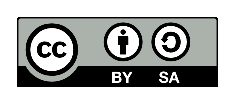
\includegraphics[scale=0.5]{img/cc-by-sa_88x31} \par
	{\footnotesize{This work is licensed under the Creative Commons Attribution-ShareAlike 4.0 International License. To view a copy of this license, visit \href{http://creativecommons.org/licenses/by-sa/4.0/}{http://creativecommons.org/licenses/by-sa/4.0/} or send a letter to Creative Commons, PO Box 1866, Mountain View, CA 94042, USA.}}\par
\end{center}
\vspace*{\stretch{1}}
\newpage

%	Showing indexes
\checkodd
%\vspace*{\stretch{3}}
%\songchapter{Indexes}
%\vspace*{\stretch{5}}
%\newpage
\showindex[2]{Canti per la Liturgia, per le Celebrazioni e per la Preghiera}{chiesa}
\showindex[2]{Party}{party}
\showindex[2]{Christmas}{christmas}

%	New chapter
%	Start on a right page and the title is in a blank page
\checkodd
\vspace*{\stretch{3}}
\songchapter{Canti per la Liturgia, per le Celebrazioni e per la Preghiera}
\vspace*{\stretch{5}}
\newpage
%	Songs of this chapter
\begin{songs}{chiesa}
	%	Songs of the chiesa chapter
\input{"tex/chiesa/Adoro Te"}
\beginsong{Alleluia questa Tua parola}[
cr={\centering{\href{https://github.com/PietroPrandini/GuitarHub}{https://github.com/PietroPrandini/GuitarHub} \href{http://creativecommons.org/licenses/by-sa/4.0/}{CC-BY-SA} \filemodprintdate{\jobname}}}
]
\transpose{0}
%{\nolyrics Intro: }

\ifchorded
\beginverse*
{\nolyrics Intro: \[D] \[Em] \[G] \[D]}
\endverse
\fi

\beginchorus
\[D]Alleluia, \[A]Alleluia, \[Bm]Alleluia, A\[F#]lleluia,
\[G]Alleluia, \[D]Alleluia, \[E]Alleluia, A\[A4]lle\[A]luia.
\[D]Alleluia, \[A]Alleluia, \[Bm]Alleluia, A\[F#]lleluia,
\[G]Alleluia, \[D]Alleluia, \[E]Alleluia, A\[A4]lle\[A]lui\[D]a.
\endchorus

\beginverse*
\[D]Questa Tua parola \[C]non avr\`a mai fine,
\[G]ha varcato i cieli e \[D]porter\`a i suoi frutti.
\[D]Questa Tua parola \[C]non avr\`a mai fine,
\[G]ha varcato i cieli e \[A4]porter\`a i suoi \[A7]frutti.
\endverse

\beginchorus
\[D]Alleluia, \[A]Alleluia, \[Bm]Alleluia, A\[F#]lleluia,
\[G]Alleluia, \[D]Alleluia, \[E]Alleluia, A\[A4]lle\[A]lui\[D]a.
\endchorus

\endsong

% Copyright 2018-2022 Pietro Prandini
% 
% This file is part of GuitarHub.
% 
% GuitarHub is free software: you can redistribute it and/or modify
% it under the terms of the GNU General Public License as published by
% the Free Software Foundation, either version 3 of the License, or
% (at your option) any later version.
% 
% GuitarHub is distributed in the hope that it will be useful,
% but WITHOUT ANY WARRANTY; without even the implied warranty of
% MERCHANTABILITY or FITNESS FOR A PARTICULAR PURPOSE.  See the
% GNU General Public License for more details.
% 
% You should have received a copy of the GNU General Public License
% along with GuitarHub.  If not, see <https://www.gnu.org/licenses/>.

\ifchorded

  \beginverse* 
  {\nolyrics Intro: \[Dm] \[C] \[B&] \[A]}
  \endverse

\fi

\beginverse\memorize 
\[Dm]Nebbia e freddo, giorni lunghi e \[C]amari,
mentre il seme m\[Dm]uore.
\[F]Poi il prodigio, antico e sempre \[C]nuovo
del primo filo d'\[B&]erba, e nel \[F]vento
dell'es\[C]tate ond\[Dm]eggiano le \[F]spighe:
a\[C]vremo ancora \[A]pan\[D]e.
\endverse

\beginchorus
\[G]Bened\[D]ici, \[G]o \[D]Signore \[C]questa o\[G]fferta
che por\[A]tiamo a Te.
\[G]Facci \[D]uno, \[Bm]come il \[F#m]Pane \[E]che anche \[G]oggi
hai \[D]dato a noi.
\endchorus

\beginverse
^Nei filari, dopo il lungo ^inverno,
fremono le ^viti.
^La rugiada avvolge nel si^lenzio
i primi tralci ^verdi, poi i ^colori
dell'aut^unno, coi ^grappoli ^maturi:
a^vremo ancora ^vi^no.
\endverse


\beginsong{%Titles
Benedici o Signore
}[
%by={},%authors, composers, and other contributors
,cr={\centering{\href{https://github.com/PietroPrandini/GuitarHub}{https://github.com/PietroPrandini/GuitarHub} \href{http://creativecommons.org/licenses/by-sa/4.0/}{CC-BY-SA} \filemodprintdate{"tex/chiesa/Benedici o Signore -2 capo1.tex"}}}, % Copyright information
%sr={},%related scripture references
%index={V1},%an extra index entry for a line of lyrics
%ititle={V1}%an extra index entry for a hidden title
]

\capo{1}
\transpose{9}

\ifchorded
  \beginverse* % * not count the verse
	  {\nolyrics Intro: \[Dm] \[C] \[B&] \[A]}
  \endverse
\fi
	\beginverse\memorize % \memorize is used to set the chords you would like to use with ^ in the next verses
	%verse
	\[Dm]Nebbia e freddo, giorni lunghi e \[C]amari,
	mentre il seme m\[Dm]uore.
	\[F]Poi il prodigio, antico e sempre \[C]nuovo
	del primo filo d'\[B&]erba, e nel \[F]vento
	dell'es\[C]tate ond\[Dm]eggiano le \[F]spighe:
	a\[C]vremo ancora \[A]pan\[D]e.
	\endverse

	\beginchorus
	%chorus
	\[G]Bened\[D]ici, \[G]o \[D]Signore \[C]questa o\[G]fferta
	che por\[A]tiamo a Te.
	\[G]Facci \[D]uno, \[Bm]come il \[F#m]Pane \[E]che anche \[G]oggi
	hai \[D]dato a noi.
	\endchorus

	\beginverse
	^Nei filari, dopo il lungo ^inverno,
	fremono le ^viti.
	^La rugiada avvolge nel si^lenzio
	i primi tralci ^verdi, poi i ^colori
	dell'aut^unno, coi ^grappoli ^maturi:
	a^vremo ancora ^vi^no.
	\endverse
% \textnote{} %for notes

%                 Do     Re     Mi     Fa     Sol    La     Si
%Naturali:        \[C]   \[D]   \[E]   \[F]   \[G]   \[A]   \[B]
%Bemolli:         \[C&]  \[D&]  \[E&]  \[F&]  \[G&]  \[A&]  \[B&]
%Diesis:          \[C#]  \[D#]  \[E#]  \[F#]  \[G#]  \[A#]  \[B#]
%Minori:          \[Cm]  \[Dm]  \[Em]  \[Fm]  \[Gm]  \[Am]  \[Bm]
%Bemolli minori:  \[C&m] \[D&m] \[E&m] \[F&m] \[G&m] \[A&m] \[B&m]
%Diesis minori:   \[C#m] \[D#m] \[E#m] \[F#m] \[G#m] \[A#m] \[B#m]

\endsong

% Copyright 2018-2021 Pietro Prandini
% 
% This file is part of GuitarHub.
% 
% GuitarHub is free software: you can redistribute it and/or modify
% it under the terms of the GNU General Public License as published by
% the Free Software Foundation, either version 3 of the License, or
% (at your option) any later version.
% 
% GuitarHub is distributed in the hope that it will be useful,
% but WITHOUT ANY WARRANTY; without even the implied warranty of
% MERCHANTABILITY or FITNESS FOR A PARTICULAR PURPOSE.  See the
% GNU General Public License for more details.
% 
% You should have received a copy of the GNU General Public License
% along with GuitarHub.  If not, see <https://www.gnu.org/licenses/>.

\beginsong{Con gioia veniamo a Te}[
%by={authors, composers, and other contributors},
,cr={\centering{\href{https://github.com/PietroPrandini/GuitarHub}{https://github.com/PietroPrandini/GuitarHub}\\\href{http://creativecommons.org/licenses/by-sa/4.0/}{\textbf{CC BY-SA}} 2018-2021 Pietro Prandini}}, % Copyright information
%,sr={related scripture references}
%,index={an extra index entry for a line of lyrics}
%ititle={an extra index entry for a hidden title}
]

%\capo{0}
\transpose{0}

% Copyright 2018-2021 Pietro Prandini
% 
% This file is part of GuitarHub.
% 
% GuitarHub is free software: you can redistribute it and/or modify
% it under the terms of the GNU General Public License as published by
% the Free Software Foundation, either version 3 of the License, or
% (at your option) any later version.
% 
% GuitarHub is distributed in the hope that it will be useful,
% but WITHOUT ANY WARRANTY; without even the implied warranty of
% MERCHANTABILITY or FITNESS FOR A PARTICULAR PURPOSE.  See the
% GNU General Public License for more details.
% 
% You should have received a copy of the GNU General Public License
% along with GuitarHub.  If not, see <https://www.gnu.org/licenses/>.

\beginsong{Con gioia veniamo a Te}[
%by={authors, composers, and other contributors},
,cr={\centering{\href{https://github.com/PietroPrandini/GuitarHub}{https://github.com/PietroPrandini/GuitarHub}\\\href{http://creativecommons.org/licenses/by-sa/4.0/}{\textbf{CC BY-SA}} 2018-2021 Pietro Prandini}}, % Copyright information
%,sr={related scripture references}
%,index={an extra index entry for a line of lyrics}
%ititle={an extra index entry for a hidden title}
]

%\capo{0}
\transpose{0}

\input{"tex/songs/Con gioia veniamo a te.tex"}

\endsong


\endsong

\beginsong{Con gioia veniamo a Te}[
%by={authors, composers, and other contributors},
,cr={\centering{\href{https://github.com/PietroPrandini/GuitarHub}{https://github.com/PietroPrandini/GuitarHub} - \href{http://creativecommons.org/licenses/by-sa/4.0/}{CC-BY-SA} - \filemodprintdate{"tex/songs/Con gioia veniamo a te.tex"}}}, % Copyright information
%li={licensing information},
%sr={related scripture references},
%index={an extra index entry for a line of lyrics},
%ititle={an extra index entry for a hidden title}
]

%\capo{0}
\transpose{10}

% Copyright 2018-2021 Pietro Prandini
% 
% This file is part of GuitarHub.
% 
% GuitarHub is free software: you can redistribute it and/or modify
% it under the terms of the GNU General Public License as published by
% the Free Software Foundation, either version 3 of the License, or
% (at your option) any later version.
% 
% GuitarHub is distributed in the hope that it will be useful,
% but WITHOUT ANY WARRANTY; without even the implied warranty of
% MERCHANTABILITY or FITNESS FOR A PARTICULAR PURPOSE.  See the
% GNU General Public License for more details.
% 
% You should have received a copy of the GNU General Public License
% along with GuitarHub.  If not, see <https://www.gnu.org/licenses/>.

\beginsong{Con gioia veniamo a Te}[
%by={authors, composers, and other contributors},
,cr={\centering{\href{https://github.com/PietroPrandini/GuitarHub}{https://github.com/PietroPrandini/GuitarHub}\\\href{http://creativecommons.org/licenses/by-sa/4.0/}{\textbf{CC BY-SA}} 2018-2021 Pietro Prandini}}, % Copyright information
%,sr={related scripture references}
%,index={an extra index entry for a line of lyrics}
%ititle={an extra index entry for a hidden title}
]

%\capo{0}
\transpose{0}

\input{"tex/songs/Con gioia veniamo a te.tex"}

\endsong


\endsong

% Copyright 2018-2021 Pietro Prandini
% 
% This file is part of GuitarHub.
% 
% GuitarHub is free software: you can redistribute it and/or modify
% it under the terms of the GNU General Public License as published by
% the Free Software Foundation, either version 3 of the License, or
% (at your option) any later version.
% 
% GuitarHub is distributed in the hope that it will be useful,
% but WITHOUT ANY WARRANTY; without even the implied warranty of
% MERCHANTABILITY or FITNESS FOR A PARTICULAR PURPOSE.  See the
% GNU General Public License for more details.
% 
% You should have received a copy of the GNU General Public License
% along with GuitarHub.  If not, see <https://www.gnu.org/licenses/>.

\ifchorded

\beginverse* 
{\nolyrics Intro: \[A] \[Bm] \[F#m] \[G] \[D] \[Em] \[D]}
\endverse

\fi

\beginchorus
\[D]Del tuo \[G]Spiri\[D]to, \[G]Signo\[D]re, \[A]\'e \[Bm]piena la \[F#m]terr\[G]a,
\'e \[D]piena la \[Em]terr\[D]a. \rep{2}
\endchorus

\beginverse\memorize
\[C]Benedici il Si\[B&]gnore,
\[Dm]anima \[Am]mi\[B&]a,
Si\[C]gnore, \[F]Dio\[C],
tu sei \[G]grand\[C]e!
\[C]Sono immense, splend\[B&]enti
\[Dm]tutte le Tue o\[B&]per\[F]e
e t\[Gm]utte le crea\[Gm]tur\[D]e.
\endverse

\beginverse
^Se tu togli il tuo ^soffio
^muore ogni ^cos^a
e ^si diss^olv^e
nella ^terr^a.
^Il tuo spirito ^scende
^tutto si ^ricre^a
e t^utto si ^rinnov^a.
\endverse

\beginverse
^La tua gloria, Si^gnore,
^resti per ^sempr^e.
Gio^isci, ^Di^o,
del cr^eat^o.
^Questo semplice ^canto
^salga a te Si^gnor^e
sei ^tu la nostra gi^oi^a.
\endverse


\beginsong{%Titles
\`E giunta l'ora}[
%by={}%authors, composers, and other contributors
,cr={\centering{\href{https://github.com/PietroPrandini/GuitarHub}{https://github.com/PietroPrandini/GuitarHub}\\\href{http://creativecommons.org/licenses/by-sa/4.0/}{\textbf{CC BY-SA}} 2018-2021 Pietro Prandini}}, % Copyright information
%,sr={}%related scripture references
%,index={}%an extra index entry for a line of lyrics
%,ititle={}%an extra index entry for a hidden title
]

%\capo{0}
\transpose{0}

\beginsong{%Titles
\`E giunta l'ora}[
%by={}%authors, composers, and other contributors
,cr={\centering{\href{https://github.com/PietroPrandini/GuitarHub}{https://github.com/PietroPrandini/GuitarHub}\\\href{http://creativecommons.org/licenses/by-sa/4.0/}{\textbf{CC BY-SA}} 2018-2021 Pietro Prandini}}, % Copyright information
%,sr={}%related scripture references
%,index={}%an extra index entry for a line of lyrics
%,ititle={}%an extra index entry for a hidden title
]

%\capo{0}
\transpose{0}

\input{"tex/songs/E giunta l ora.tex"}

\endsong


\endsong

% Copyright 2018-2022 Pietro Prandini
%
% This file is part of GuitarHub.
%
% GuitarHub is free software: you can redistribute it and/or modify
% it under the terms of the GNU General Public License as published by
% the Free Software Foundation, either version 3 of the License, or
% (at your option) any later version.
%
% GuitarHub is distributed in the hope that it will be useful,
% but WITHOUT ANY WARRANTY; without even the implied warranty of
% MERCHANTABILITY or FITNESS FOR A PARTICULAR PURPOSE.  See the
% GNU General Public License for more details.
%
% You should have received a copy of the GNU General Public License
% along with GuitarHub.  If not, see <https://www.gnu.org/licenses/>.

\begin{smallsong}
\beginsong{\`E Natale}[
by={Forza venite gente}
,cr={\centering{\href{https://github.com/PietroPrandini/GuitarHub}{https://github.com/PietroPrandini/GuitarHub}\\\href{http://creativecommons.org/licenses/by-sa/4.0/}{\textbf{CC BY-SA}} 2018-2022 Pietro Prandini}}
]

\transpose{0}

% Copyright 2018-2022 Pietro Prandini
%
% This file is part of GuitarHub.
%
% GuitarHub is free software: you can redistribute it and/or modify
% it under the terms of the GNU General Public License as published by
% the Free Software Foundation, either version 3 of the License, or
% (at your option) any later version.
%
% GuitarHub is distributed in the hope that it will be useful,
% but WITHOUT ANY WARRANTY; without even the implied warranty of
% MERCHANTABILITY or FITNESS FOR A PARTICULAR PURPOSE.  See the
% GNU General Public License for more details.
%
% You should have received a copy of the GNU General Public License
% along with GuitarHub.  If not, see <https://www.gnu.org/licenses/>.

\begin{smallsong}
\beginsong{\`E Natale}[
by={Forza venite gente}
,cr={\centering{\href{https://github.com/PietroPrandini/GuitarHub}{https://github.com/PietroPrandini/GuitarHub}\\\href{http://creativecommons.org/licenses/by-sa/4.0/}{\textbf{CC BY-SA}} 2018-2022 Pietro Prandini}}
]

\transpose{0}

\input{"tex/songs/E Natale.tex"}

\endsong
\end{smallsong}


\endsong
\end{smallsong}

\beginsong{\`E Natale}[
by={Forza venite gente},
,cr={\centering{\href{https://github.com/PietroPrandini/GuitarHub}{https://github.com/PietroPrandini/GuitarHub}\\\href{http://creativecommons.org/licenses/by-sa/4.0/}{\textbf{CC BY-SA}} 2018-2021 Pietro Prandini}}, % Copyright information
%sr={related scripture references},
%index={an extra index entry for a line of lyrics},
%ititle={an extra index entry for a hidden title}
]
\transpose{10}

% Copyright 2018-2022 Pietro Prandini
%
% This file is part of GuitarHub.
%
% GuitarHub is free software: you can redistribute it and/or modify
% it under the terms of the GNU General Public License as published by
% the Free Software Foundation, either version 3 of the License, or
% (at your option) any later version.
%
% GuitarHub is distributed in the hope that it will be useful,
% but WITHOUT ANY WARRANTY; without even the implied warranty of
% MERCHANTABILITY or FITNESS FOR A PARTICULAR PURPOSE.  See the
% GNU General Public License for more details.
%
% You should have received a copy of the GNU General Public License
% along with GuitarHub.  If not, see <https://www.gnu.org/licenses/>.

\begin{smallsong}
\beginsong{\`E Natale}[
by={Forza venite gente}
,cr={\centering{\href{https://github.com/PietroPrandini/GuitarHub}{https://github.com/PietroPrandini/GuitarHub}\\\href{http://creativecommons.org/licenses/by-sa/4.0/}{\textbf{CC BY-SA}} 2018-2022 Pietro Prandini}}
]

\transpose{0}

\input{"tex/songs/E Natale.tex"}

\endsong
\end{smallsong}


\endsong

% Copyright 2018-2021 Pietro Prandini
% 
% This file is part of GuitarHub.
% 
% GuitarHub is free software: you can redistribute it and/or modify
% it under the terms of the GNU General Public License as published by
% the Free Software Foundation, either version 3 of the License, or
% (at your option) any later version.
% 
% GuitarHub is distributed in the hope that it will be useful,
% but WITHOUT ANY WARRANTY; without even the implied warranty of
% MERCHANTABILITY or FITNESS FOR A PARTICULAR PURPOSE.  See the
% GNU General Public License for more details.
% 
% You should have received a copy of the GNU General Public License
% along with GuitarHub.  If not, see <https://www.gnu.org/licenses/>.

\beginsong{\`E Natale ancora}[
,cr={\centering{\href{https://github.com/PietroPrandini/GuitarHub}{https://github.com/PietroPrandini/GuitarHub}\\\href{http://creativecommons.org/licenses/by-sa/4.0/}{\textbf{CC BY-SA}} 2018-2021 Pietro Prandini}}
]

\transpose{0}

% Copyright 2018-2021 Pietro Prandini
% 
% This file is part of GuitarHub.
% 
% GuitarHub is free software: you can redistribute it and/or modify
% it under the terms of the GNU General Public License as published by
% the Free Software Foundation, either version 3 of the License, or
% (at your option) any later version.
% 
% GuitarHub is distributed in the hope that it will be useful,
% but WITHOUT ANY WARRANTY; without even the implied warranty of
% MERCHANTABILITY or FITNESS FOR A PARTICULAR PURPOSE.  See the
% GNU General Public License for more details.
% 
% You should have received a copy of the GNU General Public License
% along with GuitarHub.  If not, see <https://www.gnu.org/licenses/>.

\beginsong{\`E Natale ancora}[
,cr={\centering{\href{https://github.com/PietroPrandini/GuitarHub}{https://github.com/PietroPrandini/GuitarHub}\\\href{http://creativecommons.org/licenses/by-sa/4.0/}{\textbf{CC BY-SA}} 2018-2021 Pietro Prandini}}
]

\transpose{0}

\input{"tex/songs/E Natale ancora.tex"}

\endsong



\endsong


% Copyright 2018-2021 Pietro Prandini
%
% This file is part of GuitarHub.
%
% GuitarHub is free software: you can redistribute it and/or modify
% it under the terms of the GNU General Public License as published by
% the Free Software Foundation, either version 3 of the License, or
% (at your option) any later version.
%
% GuitarHub is distributed in the hope that it will be useful,
% but WITHOUT ANY WARRANTY; without even the implied warranty of
% MERCHANTABILITY or FITNESS FOR A PARTICULAR PURPOSE.  See the
% GNU General Public License for more details.
%
% You should have received a copy of the GNU General Public License
% along with GuitarHub.  If not, see <https://www.gnu.org/licenses/>.

\begin{twocolssong}\begin{smallsong}
\beginsong{E sono solo un uomo}[
,cr={\centering{\href{https://github.com/PietroPrandini/GuitarHub}{https://github.com/PietroPrandini/GuitarHub}\\\href{http://creativecommons.org/licenses/by-sa/4.0/}{\textbf{CC BY-SA}} 2018-2021 Pietro Prandini}}
]

\transpose{0}

% Copyright 2018-2021 Pietro Prandini
%
% This file is part of GuitarHub.
%
% GuitarHub is free software: you can redistribute it and/or modify
% it under the terms of the GNU General Public License as published by
% the Free Software Foundation, either version 3 of the License, or
% (at your option) any later version.
%
% GuitarHub is distributed in the hope that it will be useful,
% but WITHOUT ANY WARRANTY; without even the implied warranty of
% MERCHANTABILITY or FITNESS FOR A PARTICULAR PURPOSE.  See the
% GNU General Public License for more details.
%
% You should have received a copy of the GNU General Public License
% along with GuitarHub.  If not, see <https://www.gnu.org/licenses/>.

\begin{twocolssong}\begin{smallsong}
\beginsong{E sono solo un uomo}[
,cr={\centering{\href{https://github.com/PietroPrandini/GuitarHub}{https://github.com/PietroPrandini/GuitarHub}\\\href{http://creativecommons.org/licenses/by-sa/4.0/}{\textbf{CC BY-SA}} 2018-2021 Pietro Prandini}}
]

\transpose{0}

\input{"tex/songs/E sono solo un uomo.tex"}

\endsong
\end{smallsong}\end{twocolssong}


\endsong
\end{smallsong}\end{twocolssong}

\beginsong{Eccomi}[
by={Frisina}
,cr={\centering{\href{https://github.com/PietroPrandini/GuitarHub}{https://github.com/PietroPrandini/GuitarHub} - \href{http://creativecommons.org/licenses/by-sa/4.0/}{CC-BY-SA} - \filemodprintdate{"tex/songsBodies/Eccomi.tex"}}}, % Copyright information
]
\transpose{2}

\beginsong{Eccomi}[
by={Frisina}
,cr={\centering{\href{https://github.com/PietroPrandini/GuitarHub}{https://github.com/PietroPrandini/GuitarHub} - \href{http://creativecommons.org/licenses/by-sa/4.0/}{CC-BY-SA} - \filemodprintdate{"tex/songsBodies/Eccomi.tex"}}}, % Copyright information
]
\transpose{2}

\input{"tex/songsBodies/Eccomi.tex"}

\endsong


\endsong

% Copyright 2018-2021 Pietro Prandini
% 
% This file is part of GuitarHub.
% 
% GuitarHub is free software: you can redistribute it and/or modify
% it under the terms of the GNU General Public License as published by
% the Free Software Foundation, either version 3 of the License, or
% (at your option) any later version.
% 
% GuitarHub is distributed in the hope that it will be useful,
% but WITHOUT ANY WARRANTY; without even the implied warranty of
% MERCHANTABILITY or FITNESS FOR A PARTICULAR PURPOSE.  See the
% GNU General Public License for more details.
% 
% You should have received a copy of the GNU General Public License
% along with GuitarHub.  If not, see <https://www.gnu.org/licenses/>.

\beginsong{Eccomi}[
by={Frisina}
,cr={\centering{\href{https://github.com/PietroPrandini/GuitarHub}{https://github.com/PietroPrandini/GuitarHub}\\\href{http://creativecommons.org/licenses/by-sa/4.0/}{\textbf{CC BY-SA}} 2018-2021 Pietro Prandini}}
]

\transpose{0}

\beginsong{Eccomi}[
by={Frisina}
,cr={\centering{\href{https://github.com/PietroPrandini/GuitarHub}{https://github.com/PietroPrandini/GuitarHub} - \href{http://creativecommons.org/licenses/by-sa/4.0/}{CC-BY-SA} - \filemodprintdate{"tex/songsBodies/Eccomi.tex"}}}, % Copyright information
]
\transpose{2}

\input{"tex/songsBodies/Eccomi.tex"}

\endsong


\endsong


% Copyright 2018-2023 Pietro Prandini
%
% This file is part of GuitarHub.
%
% GuitarHub is free software: you can redistribute it and/or modify
% it under the terms of the GNU General Public License as published by
% the Free Software Foundation, either version 3 of the License, or
% (at your option) any later version.
%
% GuitarHub is distributed in the hope that it will be useful,
% but WITHOUT ANY WARRANTY; without even the implied warranty of
% MERCHANTABILITY or FITNESS FOR A PARTICULAR PURPOSE.  See the
% GNU General Public License for more details.
%
% You should have received a copy of the GNU General Public License
% along with GuitarHub.  If not, see <https://www.gnu.org/licenses/>.

\begin{twocolssong}
\beginsong{Eccomi}[
by={Frisina}
,cr={\centering{\href{https://github.com/PietroPrandini/GuitarHub}{https://github.com/PietroPrandini/GuitarHub}\\\href{http://creativecommons.org/licenses/by-sa/4.0/}{\textbf{CC BY-SA}} 2018-2023 Pietro Prandini}}
]

\transpose{9}

\beginsong{Eccomi}[
by={Frisina}
,cr={\centering{\href{https://github.com/PietroPrandini/GuitarHub}{https://github.com/PietroPrandini/GuitarHub} - \href{http://creativecommons.org/licenses/by-sa/4.0/}{CC-BY-SA} - \filemodprintdate{"tex/songsBodies/Eccomi.tex"}}}, % Copyright information
]
\transpose{2}

\input{"tex/songsBodies/Eccomi.tex"}

\endsong


\endsong
\end{twocolssong}

\ifchorded
  \beginverse* % * not count the verse
	  {\nolyrics Intro: \[D Bm F#m A]}
  \endverse
\fi
\beginchorus
Gloria a \[D]Dio nel\[Bm]l’alto dei \[F#m]cieli\[A],
e \[Bm]pace in terra agli \[F#m]uomini di \[G]buona volont\`a\[A].
Gloria a \[D]Dio nel\[Bm]l’alto dei \[F#m]cieli\[A],
e \[Bm]pace in terra agli \[F#m]uomini di \[G]buona volon\[D]t\`a.\[G] \[D]
\endchorus
\beginverse\memorize
\[A]Noi ti \[D]lodiamo e \[A]ti benedici\[D]amo,
\[E]noi ti ado\[A]riamo e \[E]ti glorifichia\[A]mo,
\[Bm]ti rendiamo gr\[F#m]azie per la \[G]tua gloria imme\[A]nsa,
\[Bm]Signore Dio, Re\[F#m] del Cielo, Dio \[G]Padre onni\[Em]poten\[A]te.
\endverse
\beginchorus
Gloria a \[D]Dio nel\[Bm]l’alto dei \[F#m]cieli\[A],
e \[Bm]pace in terra agli \[F#m]uomini di \[G]buona volon\[D]t\`a.\[G] \[D]
\endchorus
\beginverse
Si^gnore, Figlio Uni^genito,
Ges\`u ^Cristo, Signore ^Dio,
A^gnello di ^Dio, \[Bm]Figlio del \[A]Padre,
tu che \[Bm]togli i pecca\[F#m]ti del mondo,
\[G]abbi piet\`a di\[Em] \[A]noi.
\endverse
\beginchorus
Gloria a \[D]Dio nel\[Bm]l’alto dei \[F#m]cieli\[A],
e \[Bm]pace in terra agli \[F#m]uomini di \[G]buona volon\[D]t\`a.\[G] \[D]
\endchorus
\beginverse
Tu che ^togli i peccati del ^mondo,
ac^cogli la nostra ^supplica;
tu che ^siedi alla destra del ^Padre,
^abbi piet\`a^ di noi.
\endverse
\beginchorus
Gloria a \[D]Dio nel\[Bm]l’alto dei \[F#m]cieli\[A],
e \[Bm]pace in terra agli \[F#m]uomini di \[G]buona volon\[D]t\`a.\[G] \[D]
\endchorus
\beginverse
Per^ch\'e tu solo il ^Santo, tu ^solo il Si^gnore,
tu ^solo l’Al^tissimo, ^Cristo^ Ges\`u,
^con lo Spirito San^to:
nella ^Gloria di\[Em] Dio\[A] Padre.
\endverse
\beginchorus
Gloria a \[D]Dio nel\[Bm]l’alto dei \[F#m]cieli\[A],
e \[Bm]pace in terra agli \[F#m]uomini di \[G]buona volont\`a\[A].
Gloria a \[D]Dio nel\[Bm]l’alto dei \[F#m]cieli\[A],
e \[Bm]pace in terra agli \[F#m]uomini di \[G]buona volon\[D]t\`a.\[G] \[D]
\endchorus

% Copyright 2018-2021 Pietro Prandini
% 
% This file is part of GuitarHub.
% 
% GuitarHub is free software: you can redistribute it and/or modify
% it under the terms of the GNU General Public License as published by
% the Free Software Foundation, either version 3 of the License, or
% (at your option) any later version.
% 
% GuitarHub is distributed in the hope that it will be useful,
% but WITHOUT ANY WARRANTY; without even the implied warranty of
% MERCHANTABILITY or FITNESS FOR A PARTICULAR PURPOSE.  See the
% GNU General Public License for more details.
% 
% You should have received a copy of the GNU General Public License
% along with GuitarHub.  If not, see <https://www.gnu.org/licenses/>.

\beginsong{Gloria a Dio nell'alto dei cieli}[
by={Francesco Buttazzo}
,cr={\centering{\href{https://github.com/PietroPrandini/GuitarHub}{https://github.com/PietroPrandini/GuitarHub}\\\href{http://creativecommons.org/licenses/by-sa/4.0/}{\textbf{CC BY-SA}} 2018-2021 Pietro Prandini}}, % Copyright information
]
\transpose{10}

\ifchorded
  \beginverse* % * not count the verse
	  {\nolyrics Intro: \[D Bm F#m A]}
  \endverse
\fi
\beginchorus
Gloria a \[D]Dio nel\[Bm]l’alto dei \[F#m]cieli\[A],
e \[Bm]pace in terra agli \[F#m]uomini di \[G]buona volont\`a\[A].
Gloria a \[D]Dio nel\[Bm]l’alto dei \[F#m]cieli\[A],
e \[Bm]pace in terra agli \[F#m]uomini di \[G]buona volon\[D]t\`a.\[G] \[D]
\endchorus
\beginverse\memorize
\[A]Noi ti \[D]lodiamo e \[A]ti benedici\[D]amo,
\[E]noi ti ado\[A]riamo e \[E]ti glorifichia\[A]mo,
\[Bm]ti rendiamo gr\[F#m]azie per la \[G]tua gloria imme\[A]nsa,
\[Bm]Signore Dio, Re\[F#m] del Cielo, Dio \[G]Padre onni\[Em]poten\[A]te.
\endverse
\beginchorus
Gloria a \[D]Dio nel\[Bm]l’alto dei \[F#m]cieli\[A],
e \[Bm]pace in terra agli \[F#m]uomini di \[G]buona volon\[D]t\`a.\[G] \[D]
\endchorus
\beginverse
Si^gnore, Figlio Uni^genito,
Ges\`u ^Cristo, Signore ^Dio,
A^gnello di ^Dio, \[Bm]Figlio del \[A]Padre,
tu che \[Bm]togli i pecca\[F#m]ti del mondo,
\[G]abbi piet\`a di\[Em] \[A]noi.
\endverse
\beginchorus
Gloria a \[D]Dio nel\[Bm]l’alto dei \[F#m]cieli\[A],
e \[Bm]pace in terra agli \[F#m]uomini di \[G]buona volon\[D]t\`a.\[G] \[D]
\endchorus
\beginverse
Tu che ^togli i peccati del ^mondo,
ac^cogli la nostra ^supplica;
tu che ^siedi alla destra del ^Padre,
^abbi piet\`a^ di noi.
\endverse
\beginchorus
Gloria a \[D]Dio nel\[Bm]l’alto dei \[F#m]cieli\[A],
e \[Bm]pace in terra agli \[F#m]uomini di \[G]buona volon\[D]t\`a.\[G] \[D]
\endchorus
\beginverse
Per^ch\'e tu solo il ^Santo, tu ^solo il Si^gnore,
tu ^solo l’Al^tissimo, ^Cristo^ Ges\`u,
^con lo Spirito San^to:
nella ^Gloria di\[Em] Dio\[A] Padre.
\endverse
\beginchorus
Gloria a \[D]Dio nel\[Bm]l’alto dei \[F#m]cieli\[A],
e \[Bm]pace in terra agli \[F#m]uomini di \[G]buona volont\`a\[A].
Gloria a \[D]Dio nel\[Bm]l’alto dei \[F#m]cieli\[A],
e \[Bm]pace in terra agli \[F#m]uomini di \[G]buona volon\[D]t\`a.\[G] \[D]
\endchorus


\endsong

\beginsong{%Titles
Invochiamo la Tua presenza}[
%by={},%authors, composers, and other contributors
,cr={\centering{\href{https://github.com/PietroPrandini/GuitarHub}{https://github.com/PietroPrandini/GuitarHub}\\\href{http://creativecommons.org/licenses/by-sa/4.0/}{\textbf{CC BY-SA}} Pietro Prandini 2021}}, % Copyright information
%sr={},%related scripture references
%index={},%an extra index entry for a line of lyrics
%ititle={}%an extra index entry for a hidden title
]

%\capo{0}
\transpose{0}

\beginsong{%Titles
Invochiamo la Tua presenza}[
%by={},%authors, composers, and other contributors
,cr={\centering{\href{https://github.com/PietroPrandini/GuitarHub}{https://github.com/PietroPrandini/GuitarHub}\\\href{http://creativecommons.org/licenses/by-sa/4.0/}{\textbf{CC BY-SA}} Pietro Prandini 2021}}, % Copyright information
%sr={},%related scripture references
%index={},%an extra index entry for a line of lyrics
%ititle={}%an extra index entry for a hidden title
]

%\capo{0}
\transpose{0}

\input{"tex/songs/Invochiamo la Tua presenza.tex"}

\endsong


\endsong

% Copyright 2018-2023 Pietro Prandini
% 
% This file is part of GuitarHub.
% 
% GuitarHub is free software: you can redistribute it and/or modify
% it under the terms of the GNU General Public License as published by
% the Free Software Foundation, either version 3 of the License, or
% (at your option) any later version.
% 
% GuitarHub is distributed in the hope that it will be useful,
% but WITHOUT ANY WARRANTY; without even the implied warranty of
% MERCHANTABILITY or FITNESS FOR A PARTICULAR PURPOSE.  See the
% GNU General Public License for more details.
% 
% You should have received a copy of the GNU General Public License
% along with GuitarHub.  If not, see <https://www.gnu.org/licenses/>.

\beginverse\memorize 
\[F]Quello che sono, \[B&]quello che ho
\[C]io lo depongo ai Tuoi \[Gm]piedi, \[F]Sign\[C]or
\[Dm]ogni mio errore \[B&]io lascio a Te
le \[Gm]gioie e i \[F]dolori io \[B&]dono a \[Gm]Te, \[C]
\endverse

\beginchorus
\[F]Io Ti offro me \[Dm]stesso e Tu
Dio della vi\[Gm]ta m\[F]ia
\[B&]cambia questo cuo\[C]re,
\[F]io Ti offro i miei \[Dm]giorni e Tu
fonte di \[Gm]santi\[F]t\`a
\[B&]ne farai una \[A]lode a \[Dm]Te, \[Am]
\[Gm]nell'offerta \[B&]di \[Gm]Ges\[F]\`u. \[C]
\endchorus

\beginverse
^Quello che fui, ^che mai sar\`o
^Ogni mio sogno e pro^getto, ^Sign^or
^Tutto in Te ^io riporr\`o
E un ^nuovo camm^ino con ^Te scopri^r\`o ^
\endverse

\beginverse*
\textnote{Bridge}
\[D&]Cosa Ti \[E&]diamo che \[Cm]non sia Tuo dono\[Fm]
\[B&m]e cosa a\[E&]bbiamo che \[Cm]non sia gi\`a \[Fm]Tuo
\[B&m]Ogni crea\[E&]tura \[Cm]vivendo c\[F]anti
\[B&m]Le Tue mera\[A&]viglie, Sig\[B&]nor\[C]
\endverse


% Copyright 2018-2021 Pietro Prandini
% 
% This file is part of GuitarHub.
% 
% GuitarHub is free software: you can redistribute it and/or modify
% it under the terms of the GNU General Public License as published by
% the Free Software Foundation, either version 3 of the License, or
% (at your option) any later version.
% 
% GuitarHub is distributed in the hope that it will be useful,
% but WITHOUT ANY WARRANTY; without even the implied warranty of
% MERCHANTABILITY or FITNESS FOR A PARTICULAR PURPOSE.  See the
% GNU General Public License for more details.
% 
% You should have received a copy of the GNU General Public License
% along with GuitarHub.  If not, see <https://www.gnu.org/licenses/>.

\beginsong{Io ti offro}[
,cr={\centering{\href{https://github.com/PietroPrandini/GuitarHub}{https://github.com/PietroPrandini/GuitarHub}\\\href{http://creativecommons.org/licenses/by-sa/4.0/}{\textbf{CC BY-SA}} 2018-2021 Pietro Prandini}}
]

\transpose{11}

% Copyright 2018-2023 Pietro Prandini
% 
% This file is part of GuitarHub.
% 
% GuitarHub is free software: you can redistribute it and/or modify
% it under the terms of the GNU General Public License as published by
% the Free Software Foundation, either version 3 of the License, or
% (at your option) any later version.
% 
% GuitarHub is distributed in the hope that it will be useful,
% but WITHOUT ANY WARRANTY; without even the implied warranty of
% MERCHANTABILITY or FITNESS FOR A PARTICULAR PURPOSE.  See the
% GNU General Public License for more details.
% 
% You should have received a copy of the GNU General Public License
% along with GuitarHub.  If not, see <https://www.gnu.org/licenses/>.

\beginverse\memorize 
\[F]Quello che sono, \[B&]quello che ho
\[C]io lo depongo ai Tuoi \[Gm]piedi, \[F]Sign\[C]or
\[Dm]ogni mio errore \[B&]io lascio a Te
le \[Gm]gioie e i \[F]dolori io \[B&]dono a \[Gm]Te, \[C]
\endverse

\beginchorus
\[F]Io Ti offro me \[Dm]stesso e Tu
Dio della vi\[Gm]ta m\[F]ia
\[B&]cambia questo cuo\[C]re,
\[F]io Ti offro i miei \[Dm]giorni e Tu
fonte di \[Gm]santi\[F]t\`a
\[B&]ne farai una \[A]lode a \[Dm]Te, \[Am]
\[Gm]nell'offerta \[B&]di \[Gm]Ges\[F]\`u. \[C]
\endchorus

\beginverse
^Quello che fui, ^che mai sar\`o
^Ogni mio sogno e pro^getto, ^Sign^or
^Tutto in Te ^io riporr\`o
E un ^nuovo camm^ino con ^Te scopri^r\`o ^
\endverse

\beginverse*
\textnote{Bridge}
\[D&]Cosa Ti \[E&]diamo che \[Cm]non sia Tuo dono\[Fm]
\[B&m]e cosa a\[E&]bbiamo che \[Cm]non sia gi\`a \[Fm]Tuo
\[B&m]Ogni crea\[E&]tura \[Cm]vivendo c\[F]anti
\[B&m]Le Tue mera\[A&]viglie, Sig\[B&]nor\[C]
\endverse



\endsong


\beginsong{%Titles
La mia anima canta}[
%by={}%authors, composers, and other contributors
,cr={\centering{\href{https://github.com/PietroPrandini/GuitarHub}{https://github.com/PietroPrandini/GuitarHub} \href{http://creativecommons.org/licenses/by-sa/4.0/}{CC-BY-SA} \filemodprintdate{\jobname}}}
%,sr={}%related scripture references
%,index={}%an extra index entry for a line of lyrics
%,ititle={}%an extra index entry for a hidden title
]

%\capo{0}
\transpose{0}

%	\beginverse* % * not count the verse
%		{\nolyrics Intro: }
%	\endverse

%	\beginverse\memorize % \memorize is used to set the chords you would like to use with ^ in the next verses
		%verse
%	\endverse

	\beginchorus
		%chorus
		\[C]La mia \[D]anima \[G]canta la gran\[Em]dezza del S\[Am]ignore,
		il mio \[B7]spirito e\[C]sulta nel \[D]mio Sal\[G]vatore.
		\[C]Nella \[D]mia po\[G]vert\`a l'\[Em]Infinito mi ha \[Am]guardata,
		in \[B7]eterno ogni cre\[C]atura mi chia\[D]mer\`a b\[G]eata.
	\endchorus

	\beginverse\memorize
		La mia g\[Am]ioia \`e nel Si\[Bm]gnore
		che \[C]ha compiuto grandi\[Bm] cose in me.
		La mia \[Am]lode al Dio \[Bm]fedele
		che \[C]ha soccorso il suo\[Bm] popolo
		e non \[G]ha dimenticato
		le s\[C]ue pro\[Cm]messe d’\[Dm]amo\[G]re.
	\endverse

	\beginverse
		Ha dis^perso i su^perbi
		nei ^pensieri inconfe^ssabili,
		ha ^deposto i po^tenti,
		ha ^risollevato gli ^umili,
		ha saz^iato gli affamati
		e ^ha aperto ai ^ricchi le ^man^i.
	\endverse
%	\textnote{} %for notes

%                 Do     Re     Mi     Fa     Sol    La     Si
%Naturali:        \[C]   \[D]   \[E]   \[F]   \[G]   \[A]   \[B]
%Bemolli:         \[C&]  \[D&]  \[E&]  \[F&]  \[G&]  \[A&]  \[B&]
%Diesis:          \[C#]  \[D#]  \[E#]  \[F#]  \[G#]  \[A#]  \[B#]
%Minori:          \[Cm]  \[Dm]  \[Em]  \[Fm]  \[Gm]  \[Am]  \[Bm]
%Bemolli minori:  \[C&m] \[D&m] \[E&m] \[F&m] \[G&m] \[A&m] \[B&m]
%Diesis minori:   \[C#m] \[D#m] \[E#m] \[F#m] \[G#m] \[A#m] \[B#m]

\endsong

\beginsong{%Titles
La mia anima canta}[
%by={}%authors, composers, and other contributors
,cr={\centering{\href{https://github.com/PietroPrandini/GuitarHub}{https://github.com/PietroPrandini/GuitarHub} \href{http://creativecommons.org/licenses/by-sa/4.0/}{CC-BY-SA} \filemodprintdate{\jobname}}}
%,sr={}%related scripture references
%,index={}%an extra index entry for a line of lyrics
%,ititle={}%an extra index entry for a hidden title
]

%\capo{0}
\transpose{10}

%	\beginverse* % * not count the verse
%		{\nolyrics Intro: }
%	\endverse

%	\beginverse\memorize % \memorize is used to set the chords you would like to use with ^ in the next verses
		%verse
%	\endverse

	\beginchorus
		%chorus
		\[C]La mia \[D]anima \[G]canta la gran\[Em]dezza del S\[Am]ignore,
		il mio \[B7]spirito e\[C]sulta nel \[D]mio Sal\[G]vatore.
		\[C]Nella \[D]mia po\[G]vert\`a l'\[Em]Infinito mi ha \[Am]guardata,
		in \[B7]eterno ogni cre\[C]atura mi chia\[D]mer\`a b\[G]eata.
	\endchorus

	\beginverse\memorize
		La mia g\[Am]ioia \`e nel Si\[Bm]gnore
		che \[C]ha compiuto grandi\[Bm] cose in me.
		La mia \[Am]lode al Dio \[Bm]fedele
		che \[C]ha soccorso il suo\[Bm] popolo
		e non \[G]ha dimenticato
		le s\[C]ue pro\[Cm]messe d’\[Dm]amo\[G]re.
	\endverse

	\beginverse
		Ha dis^perso i su^perbi
		nei ^pensieri inconfe^ssabili,
		ha ^deposto i po^tenti,
		ha ^risollevato gli ^umili,
		ha saz^iato gli affamati
		e ^ha aperto ai ^ricchi le ^man^i.
	\endverse
%	\textnote{} %for notes

%                 Do     Re     Mi     Fa     Sol    La     Si
%Naturali:        \[C]   \[D]   \[E]   \[F]   \[G]   \[A]   \[B]
%Bemolli:         \[C&]  \[D&]  \[E&]  \[F&]  \[G&]  \[A&]  \[B&]
%Diesis:          \[C#]  \[D#]  \[E#]  \[F#]  \[G#]  \[A#]  \[B#]
%Minori:          \[Cm]  \[Dm]  \[Em]  \[Fm]  \[Gm]  \[Am]  \[Bm]
%Bemolli minori:  \[C&m] \[D&m] \[E&m] \[F&m] \[G&m] \[A&m] \[B&m]
%Diesis minori:   \[C#m] \[D#m] \[E#m] \[F#m] \[G#m] \[A#m] \[B#m]

\endsong

\beginsong{%Titles
Lode e gloria a Te}[
%by={},%authors, composers, and other contributors
%cr={},%copyright information
%li={},%licensing information
%sr={},%related scripture references
%index={},%an extra index entry for a line of lyrics
%ititle={}%an extra index entry for a hidden title
]

%\capo{0}
\transpose{0}

	\beginverse* % * not count the verse
		{\nolyrics Intro: \[E] \[A] \[E] \[A]}
	\endverse
	
	\beginchorus
		%chorus
		\[E]Lode e \[A]gloria a \[E]Te,\[A] \[E]lode e \[B]gloria a \[E]Te,\[B]
		\[C#m]luce del mat\[F#m]tino, \[E]lode e gl\[B]oria a \[E]Te.\[B]
	\endchorus

	\beginverse\memorize % \memorize is used to set the chords you would like to use with ^ in the next verses
		%verse
		\[E]M'ha fatto \[A]cammin\[E]are,\[A] \[E]m'ha fatto \[B]cammin\[E]are\[B]
		\[C#m]Per questo \[F#m]canto: \[E]lode e gl\[B]oria a \[E]Te.\[B]  
	\endverse
	
	\beginverse
		^Lo lode^r\`o nel ^tempio,^ ^lo lode^r\`o nel ^ciel^
		^Per sempre ^canto: ^lode e gl^oria a ^Te.^  
	\endverse
	
	\beginverse
		^Lo lode^r\`o con ^l'arpa,^ ^io lod^er\`o il Si^gnor^
		^Mi ha fatto grandi ^cose, ^glori^a a ^Te.^ 
	\endverse
	
	\beginverse
		^Lo lode^r\`o con ^danze,^ ^mi ha fatto ^cammin^ar^
		^Per questo ^canto: ^lode e gl^oria a ^Te.^          
	\endverse
	
%	\textnote{} %for notes

%                 Do     Re     Mi     Fa     Sol    La     Si
%Naturali:        \[C]   \[D]   \[E]   \[F]   \[G]   \[A]   \[B]
%Bemolli:         \[C&]  \[D&]  \[E&]  \[F&]  \[G&]  \[A&]  \[B&]
%Diesis:          \[C#]  \[D#]  \[E#]  \[F#]  \[G#]  \[A#]  \[B#]
%Minori:          \[Cm]  \[Dm]  \[Em]  \[Fm]  \[Gm]  \[Am]  \[Bm]
%Bemolli minori:  \[C&m] \[D&m] \[E&m] \[F&m] \[G&m] \[A&m] \[B&m]
%Diesis minori:   \[C#m] \[D#m] \[E#m] \[F#m] \[G#m] \[A#m] \[B#m]

\endsong

\beginsong{Luce che sorgi}[
%by={authors, composers, and other contributors},
,cr={\centering{\href{https://github.com/PietroPrandini/GuitarHub}{https://github.com/PietroPrandini/GuitarHub}\\\href{http://creativecommons.org/licenses/by-sa/4.0/}{\textbf{CC BY-SA}} 2018-2021 Pietro Prandini}}, % Copyright information
%sr={related scripture references},
%index={an extra index entry for a line of lyrics},
%ititle={an extra index entry for a hidden title}
]

%\capo{0}
\transpose{0}

\beginsong{Luce che sorgi}[
%by={authors, composers, and other contributors},
,cr={\centering{\href{https://github.com/PietroPrandini/GuitarHub}{https://github.com/PietroPrandini/GuitarHub}\\\href{http://creativecommons.org/licenses/by-sa/4.0/}{\textbf{CC BY-SA}} 2018-2021 Pietro Prandini}}, % Copyright information
%sr={related scripture references},
%index={an extra index entry for a line of lyrics},
%ititle={an extra index entry for a hidden title}
]

%\capo{0}
\transpose{0}

\input{"tex/songs/Luce che sorgi.tex"}

\endsong


\endsong

%  \beginverse* % * not count the verse
%	  {\nolyrics Intro: \[E B C#m A B E]
%	  \[B A B]}
%  \endverse

	\beginverse\memorize % \memorize is used to set the chords you would like to use with ^ in the next verses
	  \[E]A chi \[B]\`e nell'ang\[C#m]oscia\[A] Tu \[B]dir\[E]ai: non \[B]devi \[A]teme\[B]re,
	  \[E]il tuo \[B]Signore \`e \[C#m] qui, con la \[A]forza\[B] Sua.\[E]
	  Quando in\[B]vochi il Suo \[A]nom\[B]e,\[A] Lui \[B]ti sa\[E]lver\`a.
	\endverse

	\beginchorus
	  \[E]Lui verr\`a e ti \[A]sa\[B]lve\[E]r\`a
	  Dio verr\`a e ti \[A]sa\[B]lve\[C#m]r\`a
	  di a chi \`e smar\[A]rito che certo Lui to\[B]rner\`a
	  Dio verr\`a e ti \[A]sa\[B]lve\[E]r\`a,
	  Lui verr\`a e ti \[A]sa\[B]lve\[E]r\`a,
	  Dio verr\`a e ti \[A]sa\[B]lve\[C#m]r\`a,
	  alza i tuoi o\[A]cchi a lui presto rit\[B]orner\`a
	  Lui verr\`a e ti \[A]sa\[B]lve\[E]r\`a.
	\endchorus

	\beginverse
	  ^A chi ^ha il cuo^re fer^ito tu ^dir^ai: con^fida ^in ^Dio,
	  ^il tuo ^Signore \`e ^ qui, col ^suo gra^nde amore^.
	  Quando in^vochi il Suo ^nom^e,^ Lui ^ti sa^lver\`a.
	\endverse


	\beginchorus
	  \[E]Lui verr\`a e ti \[A]sa\[B]lve\[E]r\`a
	  Dio verr\`a e ti \[A]sa\[B]lve\[C#m]r\`a
	  di a chi \`e smar\[A]rito che certo Lui to\[B]rner\`a
	  Dio verr\`a e ti \[A]sa\[B]lve\[E]r\`a,
	  Lui verr\`a e ti \[A]sa\[B]lve\[E]r\`a,
	  Dio verr\`a e ti \[A]sa\[B]lve\[C#m]r\`a,
	  alza i tuoi o\[A]cchi a lui presto rit\[B]orner\`a
	  Lui verr\`a e ti \[A]sa\[B]lve\[E]r\`a.
	\endchorus

	\beginverse
	  \[C#m]Egli \`e rifugio nelle \[B]avver\[E]sit\`a,
	  dalla temp\[F#m]esta ti riparer\`a,
	  \[E]\`e il tuo baluardo e ti\[A] difender\[F#m]\`a,
	  la forza sua \[B]Lui ti dar\`a.\[C#&]
	\endverse
	\transpose{1}
	\prefersharps
	\beginchorus
	  \[E]Lui verr\`a e ti \[A]sa\[B]lve\[E]r\`a
	  Dio verr\`a e ti \[A]sa\[B]lve\[C#m]r\`a
	  di a chi \`e smar\[A]rito che certo Lui to\[B]rner\`a
	  Dio verr\`a e ti \[A]sa\[B]lve\[E]r\`a,
	  Lui verr\`a e ti \[A]sa\[B]lve\[E]r\`a,
	  Dio verr\`a e ti \[A]sa\[B]lve\[C#m]r\`a,
	  \lrep alza i tuoi o\[A]cchi a lui presto rit\[B]orner\`a
	  Lui verr\`a e ti \[A]sa\[B]lve\[E]r\`a.\rrep \rep{3}
	\endchorus

%	\beginchorus
	%chorus
%	\endchorus

% \textnote{} %for notes

%                 Do     Re     Mi     Fa     Sol    La     Si
%Naturali:        \[C]   \[D]   \[E]   \[F]   \[G]   \[A]   \[B]
%Bemolli:         \[C&]  \[D&]  \[E&]  \[F&]  \[G&]  \[A&]  \[B&]
%Diesis:          \[C#]  \[D#]  \[E#]  \[F#]  \[G#]  \[A#]  \[B#]
%Minori:          \[Cm]  \[Dm]  \[Em]  \[Fm]  \[Gm]  \[Am]  \[Bm]
%Bemolli minori:  \[C&m] \[D&m] \[E&m] \[F&m] \[G&m] \[A&m] \[B&m]
%Diesis minori:   \[C#m] \[D#m] \[E#m] \[F#m] \[G#m] \[A#m] \[B#m]

% Copyright 2018-2022 Pietro Prandini
%
% This file is part of GuitarHub.
%
% GuitarHub is free software: you can redistribute it and/or modify
% it under the terms of the GNU General Public License as published by
% the Free Software Foundation, either version 3 of the License, or
% (at your option) any later version.
%
% GuitarHub is distributed in the hope that it will be useful,
% but WITHOUT ANY WARRANTY; without even the implied warranty of
% MERCHANTABILITY or FITNESS FOR A PARTICULAR PURPOSE.  See the
% GNU General Public License for more details.
%
% You should have received a copy of the GNU General Public License
% along with GuitarHub.  If not, see <https://www.gnu.org/licenses/>.

\begin{twocolssong}
\beginsong{Lui verr\`a e ti salver\`a}[
,cr={\centering{\href{https://github.com/PietroPrandini/GuitarHub}{https://github.com/PietroPrandini/GuitarHub}\\\href{http://creativecommons.org/licenses/by-sa/4.0/}{\textbf{CC BY-SA}} 2018-2022 Pietro Prandini}}
]

\transpose{10}

%  \beginverse* % * not count the verse
%	  {\nolyrics Intro: \[E B C#m A B E]
%	  \[B A B]}
%  \endverse

	\beginverse\memorize % \memorize is used to set the chords you would like to use with ^ in the next verses
	  \[E]A chi \[B]\`e nell'ang\[C#m]oscia\[A] Tu \[B]dir\[E]ai: non \[B]devi \[A]teme\[B]re,
	  \[E]il tuo \[B]Signore \`e \[C#m] qui, con la \[A]forza\[B] Sua.\[E]
	  Quando in\[B]vochi il Suo \[A]nom\[B]e,\[A] Lui \[B]ti sa\[E]lver\`a.
	\endverse

	\beginchorus
	  \[E]Lui verr\`a e ti \[A]sa\[B]lve\[E]r\`a
	  Dio verr\`a e ti \[A]sa\[B]lve\[C#m]r\`a
	  di a chi \`e smar\[A]rito che certo Lui to\[B]rner\`a
	  Dio verr\`a e ti \[A]sa\[B]lve\[E]r\`a,
	  Lui verr\`a e ti \[A]sa\[B]lve\[E]r\`a,
	  Dio verr\`a e ti \[A]sa\[B]lve\[C#m]r\`a,
	  alza i tuoi o\[A]cchi a lui presto rit\[B]orner\`a
	  Lui verr\`a e ti \[A]sa\[B]lve\[E]r\`a.
	\endchorus

	\beginverse
	  ^A chi ^ha il cuo^re fer^ito tu ^dir^ai: con^fida ^in ^Dio,
	  ^il tuo ^Signore \`e ^ qui, col ^suo gra^nde amore^.
	  Quando in^vochi il Suo ^nom^e,^ Lui ^ti sa^lver\`a.
	\endverse


	\beginchorus
	  \[E]Lui verr\`a e ti \[A]sa\[B]lve\[E]r\`a
	  Dio verr\`a e ti \[A]sa\[B]lve\[C#m]r\`a
	  di a chi \`e smar\[A]rito che certo Lui to\[B]rner\`a
	  Dio verr\`a e ti \[A]sa\[B]lve\[E]r\`a,
	  Lui verr\`a e ti \[A]sa\[B]lve\[E]r\`a,
	  Dio verr\`a e ti \[A]sa\[B]lve\[C#m]r\`a,
	  alza i tuoi o\[A]cchi a lui presto rit\[B]orner\`a
	  Lui verr\`a e ti \[A]sa\[B]lve\[E]r\`a.
	\endchorus

	\beginverse
	  \[C#m]Egli \`e rifugio nelle \[B]avver\[E]sit\`a,
	  dalla temp\[F#m]esta ti riparer\`a,
	  \[E]\`e il tuo baluardo e ti\[A] difender\[F#m]\`a,
	  la forza sua \[B]Lui ti dar\`a.\[C#&]
	\endverse
	\transpose{1}
	\prefersharps
	\beginchorus
	  \[E]Lui verr\`a e ti \[A]sa\[B]lve\[E]r\`a
	  Dio verr\`a e ti \[A]sa\[B]lve\[C#m]r\`a
	  di a chi \`e smar\[A]rito che certo Lui to\[B]rner\`a
	  Dio verr\`a e ti \[A]sa\[B]lve\[E]r\`a,
	  Lui verr\`a e ti \[A]sa\[B]lve\[E]r\`a,
	  Dio verr\`a e ti \[A]sa\[B]lve\[C#m]r\`a,
	  \lrep alza i tuoi o\[A]cchi a lui presto rit\[B]orner\`a
	  Lui verr\`a e ti \[A]sa\[B]lve\[E]r\`a.\rrep \rep{3}
	\endchorus

%	\beginchorus
	%chorus
%	\endchorus

% \textnote{} %for notes

%                 Do     Re     Mi     Fa     Sol    La     Si
%Naturali:        \[C]   \[D]   \[E]   \[F]   \[G]   \[A]   \[B]
%Bemolli:         \[C&]  \[D&]  \[E&]  \[F&]  \[G&]  \[A&]  \[B&]
%Diesis:          \[C#]  \[D#]  \[E#]  \[F#]  \[G#]  \[A#]  \[B#]
%Minori:          \[Cm]  \[Dm]  \[Em]  \[Fm]  \[Gm]  \[Am]  \[Bm]
%Bemolli minori:  \[C&m] \[D&m] \[E&m] \[F&m] \[G&m] \[A&m] \[B&m]
%Diesis minori:   \[C#m] \[D#m] \[E#m] \[F#m] \[G#m] \[A#m] \[B#m]


\endsong
\end{twocolssong}

% Copyright 2018-2021 Pietro Prandini
% 
% This file is part of GuitarHub.
% 
% GuitarHub is free software: you can redistribute it and/or modify
% it under the terms of the GNU General Public License as published by
% the Free Software Foundation, either version 3 of the License, or
% (at your option) any later version.
% 
% GuitarHub is distributed in the hope that it will be useful,
% but WITHOUT ANY WARRANTY; without even the implied warranty of
% MERCHANTABILITY or FITNESS FOR A PARTICULAR PURPOSE.  See the
% GNU General Public License for more details.
% 
% You should have received a copy of the GNU General Public License
% along with GuitarHub.  If not, see <https://www.gnu.org/licenses/>.

\beginsong{Magnificat}[
by={Taiz\`e}
,cr={\centering{\href{https://github.com/PietroPrandini/GuitarHub}{https://github.com/PietroPrandini/GuitarHub}\\\href{http://creativecommons.org/licenses/by-sa/4.0/}{\textbf{CC BY-SA}} 2018-2021 Pietro Prandini}}
]

\transpose{2}

% Copyright 2018-2021 Pietro Prandini
% 
% This file is part of GuitarHub.
% 
% GuitarHub is free software: you can redistribute it and/or modify
% it under the terms of the GNU General Public License as published by
% the Free Software Foundation, either version 3 of the License, or
% (at your option) any later version.
% 
% GuitarHub is distributed in the hope that it will be useful,
% but WITHOUT ANY WARRANTY; without even the implied warranty of
% MERCHANTABILITY or FITNESS FOR A PARTICULAR PURPOSE.  See the
% GNU General Public License for more details.
% 
% You should have received a copy of the GNU General Public License
% along with GuitarHub.  If not, see <https://www.gnu.org/licenses/>.

\beginsong{Magnificat}[
by={Taiz\`e}
,cr={\centering{\href{https://github.com/PietroPrandini/GuitarHub}{https://github.com/PietroPrandini/GuitarHub}\\\href{http://creativecommons.org/licenses/by-sa/4.0/}{\textbf{CC BY-SA}} 2018-2021 Pietro Prandini}}
]

\transpose{2}

\input{"tex/songs/Magnificat Taize.tex"}

\endsong



\endsong


% Copyright 2018-2023 Pietro Prandini
%
% This file is part of GuitarHub.
%
% GuitarHub is free software: you can redistribute it and/or modify
% it under the terms of the GNU General Public License as published by
% the Free Software Foundation, either version 3 of the License, or
% (at your option) any later version.
%
% GuitarHub is distributed in the hope that it will be useful,
% but WITHOUT ANY WARRANTY; without even the implied warranty of
% MERCHANTABILITY or FITNESS FOR A PARTICULAR PURPOSE.  See the
% GNU General Public License for more details.
%
% You should have received a copy of the GNU General Public License
% along with GuitarHub.  If not, see <https://www.gnu.org/licenses/>.

\begin{smallsong}
\beginsong{Maria porta dell'Avvento}[
,cr={\centering{\href{https://github.com/PietroPrandini/GuitarHub}{https://github.com/PietroPrandini/GuitarHub}\\\href{http://creativecommons.org/licenses/by-sa/4.0/}{\textbf{CC BY-SA}} 2018-2023 Pietro Prandini}}
]

\transpose{0}

% Copyright 2018-2023 Pietro Prandini
%
% This file is part of GuitarHub.
%
% GuitarHub is free software: you can redistribute it and/or modify
% it under the terms of the GNU General Public License as published by
% the Free Software Foundation, either version 3 of the License, or
% (at your option) any later version.
%
% GuitarHub is distributed in the hope that it will be useful,
% but WITHOUT ANY WARRANTY; without even the implied warranty of
% MERCHANTABILITY or FITNESS FOR A PARTICULAR PURPOSE.  See the
% GNU General Public License for more details.
%
% You should have received a copy of the GNU General Public License
% along with GuitarHub.  If not, see <https://www.gnu.org/licenses/>.

\begin{smallsong}
\beginsong{Maria porta dell'Avvento}[
,cr={\centering{\href{https://github.com/PietroPrandini/GuitarHub}{https://github.com/PietroPrandini/GuitarHub}\\\href{http://creativecommons.org/licenses/by-sa/4.0/}{\textbf{CC BY-SA}} 2018-2023 Pietro Prandini}}
]

\transpose{0}

\input{"tex/songs/Maria porta dell Avvento.tex"}

\endsong
\end{smallsong}


\endsong
\end{smallsong}

\beginsong{%Titles
Pane del Cielo}[
%by={}%authors, composers, and other contributors
,cr={\centering{\href{https://github.com/PietroPrandini/GuitarHub}{https://github.com/PietroPrandini/GuitarHub}\\\href{http://creativecommons.org/licenses/by-sa/4.0/}{\textbf{CC BY-SA}} Pietro Prandini 2021}}, % Copyright information
%,sr={}%related scripture references
%,index={}%an extra index entry for a line of lyrics
%,ititle={}%an extra index entry for a hidden title
]

%\capo{0}
\transpose{0}

\beginsong{%Titles
Pane del Cielo}[
%by={}%authors, composers, and other contributors
,cr={\centering{\href{https://github.com/PietroPrandini/GuitarHub}{https://github.com/PietroPrandini/GuitarHub}\\\href{http://creativecommons.org/licenses/by-sa/4.0/}{\textbf{CC BY-SA}} Pietro Prandini 2021}}, % Copyright information
%,sr={}%related scripture references
%,index={}%an extra index entry for a line of lyrics
%,ititle={}%an extra index entry for a hidden title
]

%\capo{0}
\transpose{0}

\input{"tex/songs/Pane del cielo.tex"}

\endsong


\endsong

\beginsong{Santo Frisina}[
%by={Frisina}
,cr={\centering{\href{https://github.com/PietroPrandini/GuitarHub}{https://github.com/PietroPrandini/GuitarHub} \href{http://creativecommons.org/licenses/by-sa/4.0/}{CC-BY-SA} \filemodprintdate{\jobname}}}
]
\capo{1}
\transpose{11}
%{\nolyrics Intro: }
\beginverse
\[E&]Santo, \[B&]santo, \[Cm]san\[Gm7]to il Si\[A&]gnore \[E&]Dio dell'uni\[Fm]ver\[B&]so.
I \[Cm]cieli e la\[Gm] terra sono \[A&]pieni\[E&] della \[Cm]tua \[F]gl\[B&4]oria\[B&].
\endverse
\beginchorus
Ho\[E&]sanna \[B&]in ex\[Cm]cel\[Gm]sis. Ho\[A&]sanna \[E&]in ex\[B&4 B&]cel\[E&]sis.
\endchorus
\beginverse
\[G]Bene\[Cm]detto co\[A&]lui che \[G]viene nel \[Cm]nome \[A&]del Si\[B&4]gno\[B&]re.
\endverse
\beginchorus
Ho\[E&]sanna \[B&]in ex\[Cm]cel\[Gm]sis. Ho\[A&]sanna \[E&]in ex\[B&4 B&]cel\[E&]sis.
\endchorus
\endsong

\beginsong{Santo Frisina}[
%by={Frisina}
,cr={\centering{\href{https://github.com/PietroPrandini/GuitarHub}{https://github.com/PietroPrandini/GuitarHub}\\\href{http://creativecommons.org/licenses/by-sa/4.0/}{\textbf{CC BY-SA}} 2018-2021 Pietro Prandini}}, % Copyright information
]
\transpose{9}

% Copyright 2018-2023 Pietro Prandini
% 
% This file is part of GuitarHub.
% 
% GuitarHub is free software: you can redistribute it and/or modify
% it under the terms of the GNU General Public License as published by
% the Free Software Foundation, either version 3 of the License, or
% (at your option) any later version.
% 
% GuitarHub is distributed in the hope that it will be useful,
% but WITHOUT ANY WARRANTY; without even the implied warranty of
% MERCHANTABILITY or FITNESS FOR A PARTICULAR PURPOSE.  See the
% GNU General Public License for more details.
% 
% You should have received a copy of the GNU General Public License
% along with GuitarHub.  If not, see <https://www.gnu.org/licenses/>.

\beginverse
\[E&]Santo, \[B&]santo, \[Cm]san\[Gm7]to il Si\[A&]gnore \[E&]Dio dell'uni\[Fm]ver\[B&]so.
I \[Cm]cieli e la\[Gm] terra sono \[A&]pieni\[E&] della \[Cm]tua \[F]gl\[B&4]oria\[B&].
\endverse

\beginchorus
Ho\[E&]sanna \[B&]in ex\[Cm]cel\[Gm]sis. Ho\[A&]sanna \[E&]in ex\[B&4 B&]cel\[E&]sis.
\endchorus

\beginverse
\[G]Bene\[Cm]detto co\[A&]lui che \[G]viene nel \[Cm]nome \[A&]del Si\[B&4]gno\[B&]re.
\endverse

\beginchorus
Ho\[E&]sanna \[B&]in ex\[Cm]cel\[Gm]sis. Ho\[A&]sanna \[E&]in ex\[B&4 B&]cel\[E&]sis.
\endchorus



\endsong

\beginsong{%Titles
Santo Giovani}[
%by={Giovani}%authors, composers, and other contributors
,cr={\centering{\href{https://github.com/PietroPrandini/GuitarHub}{https://github.com/PietroPrandini/GuitarHub} - \href{http://creativecommons.org/licenses/by-sa/4.0/}{CC-BY-SA} - \filemodprintdate{"tex/chiesa/Santo Giovani.tex"}}}, % Copyright information
%,sr={}%related scripture references
%,index={}%an extra index entry for a line of lyrics
%,ititle={}%an extra index entry for a hidden title
]

%\capo{0}
\transpose{0}
\meter{4}{4}

	\ifchorded
	\beginverse* % * not count the verse
		{\nolyrics Intro: | \[G] \[C] | \[D] \[G] |}
	\endverse
	\fi

	\beginverse*\memorize % \memorize is used to set the chords you would like to use with ^ in the next verses
		%verse
		\[G]Santo, \[C]santo, \[D]santo il Si\[G]gnore
		\[Am]Dio dell'\[C]uni\[D4]verso.\[D]
		I \[Em]cieli \[C]e la \[D]ter\[G]ra
		sono \[Em]pieni \[C]della tua \[D4]glo\[D]ria.
	\endverse

	\beginchorus
		%chorus
		O\[C]san\[D]na, o\[G]san\[C]na,
		o\[Am]sanna ne\[C]ll'alto dei \[D4]cieli\[D].
		O\[C]san\[D]na, o\[G]san\[C]na,
		o\[Am]sanna ne\[D]ll'alto dei \[G]cieli\[G].
	\endchorus

	\ifchorded
	\beginverse* % * not count the verse
		{\nolyrics Strum: | \[Em] \[C] | \[D] \[G] }
	\endverse
	\fi

	\beginverse*
		Bene|\[Em]detto c\[C]olui che \[D4]vie\[G]ne
		nel \[Em]nome \[C]del Si\[D4]gno\[D]re.
	\endverse

	\beginchorus
		%chorus
		O\[C]san\[D]na, o\[G]san\[C]na,
		o\[Am]sanna ne\[C]ll'alto dei \[D4]cieli\[D].
		O\[C]san\[D]na, o\[G]san\[C]na,
		o\[Am]sanna ne\[D]ll'alto dei \[G]cieli\[G].
		\[C]Santo, \[D]santo, \[C]san\[C7+]to.
	\endchorus

%	\textnote{} %for notes

%                 Do     Re     Mi     Fa     Sol    La     Si
%Naturali:        \[C]   \[D]   \[E]   \[F]   \[G]   \[A]   \[B]
%Bemolli:         \[C&]  \[D&]  \[E&]  \[F&]  \[G&]  \[A&]  \[B&]
%Diesis:          \[C#]  \[D#]  \[E#]  \[F#]  \[G#]  \[A#]  \[B#]
%Minori:          \[Cm]  \[Dm]  \[Em]  \[Fm]  \[Gm]  \[Am]  \[Bm]
%Bemolli minori:  \[C&m] \[D&m] \[E&m] \[F&m] \[G&m] \[A&m] \[B&m]
%Diesis minori:   \[C#m] \[D#m] \[E#m] \[F#m] \[G#m] \[A#m] \[B#m]

\endsong

% Copyright 2018-2023 Pietro Prandini
% 
% This file is part of GuitarHub.
% 
% GuitarHub is free software: you can redistribute it and/or modify
% it under the terms of the GNU General Public License as published by
% the Free Software Foundation, either version 3 of the License, or
% (at your option) any later version.
% 
% GuitarHub is distributed in the hope that it will be useful,
% but WITHOUT ANY WARRANTY; without even the implied warranty of
% MERCHANTABILITY or FITNESS FOR A PARTICULAR PURPOSE.  See the
% GNU General Public License for more details.
% 
% You should have received a copy of the GNU General Public License
% along with GuitarHub.  If not, see <https://www.gnu.org/licenses/>.

\beginverse\memorize 
\[E]Spirito di D\[A]io riempi\[E]mi. \[A]
\[E]Spirito di D\[A]io battezza\[B]mi.
\[E]Spirito di D\[A]io cons\[E]acr\[G#]ami. \[C#m]
\[E]Vieni ad abit\[A]are dentro m\[E]e. \[A]\[E]
\endverse

\beginverse
^Spirito di D^io guarisci^mi. ^
^Spirito di D^io rinnova^mi.
^Spirito di D^io cons^acr^ami. ^
^Vieni ad abit^are dentro m^e. ^^
\endverse

\beginverse
^Spirito di D^io riempi^ci. ^
^Spirito di D^io battezza^ci.
^Spirito di D^io cons^acr^aci. ^
^Vieni ad abit^are dentro no^i. ^^
\endverse

\beginverse
^Spirito di D^io guarisci^ci. ^
^Spirito di D^io rinnova^ci.
^Spirito di D^io cons^acr^aci. ^
\lrep ^Vieni ad abit^are dentro no^i. ^^ \rrep \rep{2}
\endverse


% Copyright 2018-2021 Pietro Prandini
% 
% This file is part of GuitarHub.
% 
% GuitarHub is free software: you can redistribute it and/or modify
% it under the terms of the GNU General Public License as published by
% the Free Software Foundation, either version 3 of the License, or
% (at your option) any later version.
% 
% GuitarHub is distributed in the hope that it will be useful,
% but WITHOUT ANY WARRANTY; without even the implied warranty of
% MERCHANTABILITY or FITNESS FOR A PARTICULAR PURPOSE.  See the
% GNU General Public License for more details.
% 
% You should have received a copy of the GNU General Public License
% along with GuitarHub.  If not, see <https://www.gnu.org/licenses/>.

\beginsong{%Titles
Spirito di Dio}[
%by={}%authors, composers, and other contributors
,cr={\centering{\href{https://github.com/PietroPrandini/GuitarHub}{https://github.com/PietroPrandini/GuitarHub}\\\href{http://creativecommons.org/licenses/by-sa/4.0/}{\textbf{CC BY-SA}} 2018-2021 Pietro Prandini}}, % Copyright information
%,sr={}%related scripture references
%,index={}%an extra index entry for a line of lyrics
%ititle={Tono Note Volanti}%an extra index entry for a hidden title
]

\capo{1}
\transpose{10}

% Copyright 2018-2023 Pietro Prandini
% 
% This file is part of GuitarHub.
% 
% GuitarHub is free software: you can redistribute it and/or modify
% it under the terms of the GNU General Public License as published by
% the Free Software Foundation, either version 3 of the License, or
% (at your option) any later version.
% 
% GuitarHub is distributed in the hope that it will be useful,
% but WITHOUT ANY WARRANTY; without even the implied warranty of
% MERCHANTABILITY or FITNESS FOR A PARTICULAR PURPOSE.  See the
% GNU General Public License for more details.
% 
% You should have received a copy of the GNU General Public License
% along with GuitarHub.  If not, see <https://www.gnu.org/licenses/>.

\beginverse\memorize 
\[E]Spirito di D\[A]io riempi\[E]mi. \[A]
\[E]Spirito di D\[A]io battezza\[B]mi.
\[E]Spirito di D\[A]io cons\[E]acr\[G#]ami. \[C#m]
\[E]Vieni ad abit\[A]are dentro m\[E]e. \[A]\[E]
\endverse

\beginverse
^Spirito di D^io guarisci^mi. ^
^Spirito di D^io rinnova^mi.
^Spirito di D^io cons^acr^ami. ^
^Vieni ad abit^are dentro m^e. ^^
\endverse

\beginverse
^Spirito di D^io riempi^ci. ^
^Spirito di D^io battezza^ci.
^Spirito di D^io cons^acr^aci. ^
^Vieni ad abit^are dentro no^i. ^^
\endverse

\beginverse
^Spirito di D^io guarisci^ci. ^
^Spirito di D^io rinnova^ci.
^Spirito di D^io cons^acr^aci. ^
\lrep ^Vieni ad abit^are dentro no^i. ^^ \rrep \rep{2}
\endverse



\endsong

\beginsong{%Titles
Ti saluto o croce Santa}[
%by={}%authors, composers, and other contributors
,cr={\centering{\href{https://github.com/PietroPrandini/GuitarHub}{https://github.com/PietroPrandini/GuitarHub} - \href{http://creativecommons.org/licenses/by-sa/4.0/}{CC-BY-SA} - \filemodprintdate{"tex/chiesa/Ti saluto o croce santa.tex"}}}, % Copyright information
%,sr={}%related scripture references
%,index={}%an extra index entry for a line of lyrics
%,ititle={}%an extra index entry for a hidden title
]

%\capo{0}
\transpose{0}

%	\beginverse* % * not count the verse
%		{\nolyrics Intro: }
%	\endverse

%	\beginverse\memorize % \memorize is used to set the chords you would like to use with ^ in the next verses
		%verse
%	\endverse

	\beginchorus
		%chorus
		Ti sa\[Dm]luto, o croce \[F]Santa,
		che por\[Dm]tasti il Reden\[A]tor;
		gloria, \[F]lode, o\[Gm]nor, ti \[F]canta
		ogni \[Gm]lingua ed ogni \[Dm]cuor.
	\endchorus

	\beginverse\memorize
		\[F]Sei vessillo glorioso di Cristo,
		Sua vit\[C]toria e segno d'a\[F]mor:
		il Suo \[A]sangue innocente fu \[Dm]visto
		come \[B&]fiamma sgor\[A]gare dal \[Dm]cuor.
	\endverse

	\beginverse
		^Tu nascesti fra le braccia amorose
		d'una ^Vergine Madre, o Ge^s\`u.
		Tu mo^risti fra braccia pie^tose
		d'una ^croce che ^data ti ^fu.
	\endverse

	\beginverse
		O A^gnello divino immolato
		sull'al^tar della croce, p^iet\`a!
		Tu che ^togli dal mondo il pec^cato,
		salva l'^uomo che ^pace non ^ha.
	\endverse

	\beginverse
		Del giu^dizio nel giorno tremendo
		sulle ^nubi del cielo ver^rai:
		piange^ranno le genti ve^dendo
		qual tro^feo di g^loria sa^rai.
	\endverse

%	\textnote{} %for notes

%                 Do     Re     Mi     Fa     Sol    La     Si
%Naturali:        \[C]   \[D]   \[E]   \[F]   \[G]   \[A]   \[B]
%Bemolli:         \[C&]  \[D&]  \[E&]  \[F&]  \[G&]  \[A&]  \[B&]
%Diesis:          \[C#]  \[D#]  \[E#]  \[F#]  \[G#]  \[A#]  \[B#]
%Minori:          \[Cm]  \[Dm]  \[Em]  \[Fm]  \[Gm]  \[Am]  \[Bm]
%Bemolli minori:  \[C&m] \[D&m] \[E&m] \[F&m] \[G&m] \[A&m] \[B&m]
%Diesis minori:   \[C#m] \[D#m] \[E#m] \[F#m] \[G#m] \[A#m] \[B#m]

\endsong

% Copyright 2018-2022 Pietro Prandini
% 
% This file is part of GuitarHub.
% 
% GuitarHub is free software: you can redistribute it and/or modify
% it under the terms of the GNU General Public License as published by
% the Free Software Foundation, either version 3 of the License, or
% (at your option) any later version.
% 
% GuitarHub is distributed in the hope that it will be useful,
% but WITHOUT ANY WARRANTY; without even the implied warranty of
% MERCHANTABILITY or FITNESS FOR A PARTICULAR PURPOSE.  See the
% GNU General Public License for more details.
% 
% You should have received a copy of the GNU General Public License
% along with GuitarHub.  If not, see <https://www.gnu.org/licenses/>.

\beginsong{Ti seguir\`o}[
by={Frisina}
,cr={\centering{\href{https://github.com/PietroPrandini/GuitarHub}{https://github.com/PietroPrandini/GuitarHub}\\\href{http://creativecommons.org/licenses/by-sa/4.0/}{\textbf{CC BY-SA}} 2018-2022 Pietro Prandini}}
]

\transpose{3}

% Copyright 2018-2022 Pietro Prandini
% 
% This file is part of GuitarHub.
% 
% GuitarHub is free software: you can redistribute it and/or modify
% it under the terms of the GNU General Public License as published by
% the Free Software Foundation, either version 3 of the License, or
% (at your option) any later version.
% 
% GuitarHub is distributed in the hope that it will be useful,
% but WITHOUT ANY WARRANTY; without even the implied warranty of
% MERCHANTABILITY or FITNESS FOR A PARTICULAR PURPOSE.  See the
% GNU General Public License for more details.
% 
% You should have received a copy of the GNU General Public License
% along with GuitarHub.  If not, see <https://www.gnu.org/licenses/>.

\beginsong{Ti seguir\`o}[
by={Frisina}
,cr={\centering{\href{https://github.com/PietroPrandini/GuitarHub}{https://github.com/PietroPrandini/GuitarHub}\\\href{http://creativecommons.org/licenses/by-sa/4.0/}{\textbf{CC BY-SA}} 2018-2022 Pietro Prandini}}
]

\transpose{3}

\input{"tex/songs/Ti seguiro.tex"}

\endsong



\endsong


% Copyright 2018-2023 Pietro Prandini
% 
% This file is part of GuitarHub.
% 
% GuitarHub is free software: you can redistribute it and/or modify
% it under the terms of the GNU General Public License as published by
% the Free Software Foundation, either version 3 of the License, or
% (at your option) any later version.
% 
% GuitarHub is distributed in the hope that it will be useful,
% but WITHOUT ANY WARRANTY; without even the implied warranty of
% MERCHANTABILITY or FITNESS FOR A PARTICULAR PURPOSE.  See the
% GNU General Public License for more details.
% 
% You should have received a copy of the GNU General Public License
% along with GuitarHub.  If not, see <https://www.gnu.org/licenses/>.

\beginsong{Ti seguir\`o}[
by={Frisina}
,cr={\centering{\href{https://github.com/PietroPrandini/GuitarHub}{https://github.com/PietroPrandini/GuitarHub}\\\href{http://creativecommons.org/licenses/by-sa/4.0/}{\textbf{CC BY-SA}} 2018-2023 Pietro Prandini}}
]

\transpose{0}

% Copyright 2018-2022 Pietro Prandini
% 
% This file is part of GuitarHub.
% 
% GuitarHub is free software: you can redistribute it and/or modify
% it under the terms of the GNU General Public License as published by
% the Free Software Foundation, either version 3 of the License, or
% (at your option) any later version.
% 
% GuitarHub is distributed in the hope that it will be useful,
% but WITHOUT ANY WARRANTY; without even the implied warranty of
% MERCHANTABILITY or FITNESS FOR A PARTICULAR PURPOSE.  See the
% GNU General Public License for more details.
% 
% You should have received a copy of the GNU General Public License
% along with GuitarHub.  If not, see <https://www.gnu.org/licenses/>.

\beginsong{Ti seguir\`o}[
by={Frisina}
,cr={\centering{\href{https://github.com/PietroPrandini/GuitarHub}{https://github.com/PietroPrandini/GuitarHub}\\\href{http://creativecommons.org/licenses/by-sa/4.0/}{\textbf{CC BY-SA}} 2018-2022 Pietro Prandini}}
]

\transpose{3}

\input{"tex/songs/Ti seguiro.tex"}

\endsong



\endsong


\beginsong{%Titles
Tu Sei}[
%by={}%authors, composers, and other contributors
,cr={\centering{\href{https://github.com/PietroPrandini/GuitarHub}{https://github.com/PietroPrandini/GuitarHub} \href{http://creativecommons.org/licenses/by-sa/4.0/}{CC-BY-SA} \filemodprintdate{\jobname}}}
%,sr={}%related scripture references
%,index={}%an extra index entry for a line of lyrics
%,ititle={}%an extra index entry for a hidden title
]

%\capo{0}
%\transpose{9}

%	\beginverse* % * not count the verse
%		{\nolyrics Intro: }
%	\endverse

	\beginverse\memorize % \memorize is used to set the chords you would like to use with ^ in the next verses
		%verse
		Tu \[C]sei la prima st\[Dm]ella del mattino,
		T\[Em]u sei la nostra gra\[F]nde nostalgia,
		Tu\[Em] sei il cielo c\[Dm]hiaro \[G]dopo la \[C]paura:
		d\[G]opo la pa\[Am]ura d'esserci per\[F]duti:
		e \[Dm]torner\`a la \[C]vita in questo m\[G]are.
	\endverse

	\beginchorus
		%chorus
		Soffie\[F]r\`a, soffie\[C]r\`a il vento\[G] forte della\[Am] vita,
		soffier\`a\[F] sulle\[C] vele e le \[F]gon\[G]fier\`a di \[C]te.
		Soffie\[F]r\`a soffi\[C]er\`a il vento\[G] forte della\[Am] vita,
		so\[A&]ffier\`a sulle \[C]vele e le \[F]gon\[G]fier\`a di \[C]te.
	\endchorus

	\beginverse
		Tu ^sei l'unico vol^to della pace,
		T^u sei Speranza nelle ^nostre mani,
		Tu^ sei il vento n^uovo ^sulle nostre ^ali:
		s^ulle no^stre ali soffier\`a la ^vita
		e ^gonfier\`a le ^vele per questo m^are.
	\endverse

%	\textnote{} %for notes

%                 Do     Re     Mi     Fa     Sol    La     Si
%Naturali:        \[C]   \[D]   \[E]   \[F]   \[G]   \[A]   \[B]
%Bemolli:         \[C&]  \[D&]  \[E&]  \[F&]  \[G&]  \[A&]  \[B&]
%Diesis:          \[C#]  \[D#]  \[E#]  \[F#]  \[G#]  \[A#]  \[B#]
%Minori:          \[Cm]  \[Dm]  \[Em]  \[Fm]  \[Gm]  \[Am]  \[Bm]
%Bemolli minori:  \[C&m] \[D&m] \[E&m] \[F&m] \[G&m] \[A&m] \[B&m]
%Diesis minori:   \[C#m] \[D#m] \[E#m] \[F#m] \[G#m] \[A#m] \[B#m]

\endsong

% Copyright 2018-2022 Pietro Prandini
% 
% This file is part of GuitarHub.
% 
% GuitarHub is free software: you can redistribute it and/or modify
% it under the terms of the GNU General Public License as published by
% the Free Software Foundation, either version 3 of the License, or
% (at your option) any later version.
% 
% GuitarHub is distributed in the hope that it will be useful,
% but WITHOUT ANY WARRANTY; without even the implied warranty of
% MERCHANTABILITY or FITNESS FOR A PARTICULAR PURPOSE.  See the
% GNU General Public License for more details.
% 
% You should have received a copy of the GNU General Public License
% along with GuitarHub.  If not, see <https://www.gnu.org/licenses/>.

\beginsong{Tu Sei}[
,cr={\centering{\href{https://github.com/PietroPrandini/GuitarHub}{https://github.com/PietroPrandini/GuitarHub}\\\href{http://creativecommons.org/licenses/by-sa/4.0/}{\textbf{CC BY-SA}} 2018-2022 Pietro Prandini}}
]

\transpose{9}

\beginsong{%Titles
Tu Sei}[
%by={}%authors, composers, and other contributors
,cr={\centering{\href{https://github.com/PietroPrandini/GuitarHub}{https://github.com/PietroPrandini/GuitarHub} \href{http://creativecommons.org/licenses/by-sa/4.0/}{CC-BY-SA} \filemodprintdate{\jobname}}}
%,sr={}%related scripture references
%,index={}%an extra index entry for a line of lyrics
%,ititle={}%an extra index entry for a hidden title
]

%\capo{0}
%\transpose{9}

%	\beginverse* % * not count the verse
%		{\nolyrics Intro: }
%	\endverse

	\beginverse\memorize % \memorize is used to set the chords you would like to use with ^ in the next verses
		%verse
		Tu \[C]sei la prima st\[Dm]ella del mattino,
		T\[Em]u sei la nostra gra\[F]nde nostalgia,
		Tu\[Em] sei il cielo c\[Dm]hiaro \[G]dopo la \[C]paura:
		d\[G]opo la pa\[Am]ura d'esserci per\[F]duti:
		e \[Dm]torner\`a la \[C]vita in questo m\[G]are.
	\endverse

	\beginchorus
		%chorus
		Soffie\[F]r\`a, soffie\[C]r\`a il vento\[G] forte della\[Am] vita,
		soffier\`a\[F] sulle\[C] vele e le \[F]gon\[G]fier\`a di \[C]te.
		Soffie\[F]r\`a soffi\[C]er\`a il vento\[G] forte della\[Am] vita,
		so\[A&]ffier\`a sulle \[C]vele e le \[F]gon\[G]fier\`a di \[C]te.
	\endchorus

	\beginverse
		Tu ^sei l'unico vol^to della pace,
		T^u sei Speranza nelle ^nostre mani,
		Tu^ sei il vento n^uovo ^sulle nostre ^ali:
		s^ulle no^stre ali soffier\`a la ^vita
		e ^gonfier\`a le ^vele per questo m^are.
	\endverse

%	\textnote{} %for notes

%                 Do     Re     Mi     Fa     Sol    La     Si
%Naturali:        \[C]   \[D]   \[E]   \[F]   \[G]   \[A]   \[B]
%Bemolli:         \[C&]  \[D&]  \[E&]  \[F&]  \[G&]  \[A&]  \[B&]
%Diesis:          \[C#]  \[D#]  \[E#]  \[F#]  \[G#]  \[A#]  \[B#]
%Minori:          \[Cm]  \[Dm]  \[Em]  \[Fm]  \[Gm]  \[Am]  \[Bm]
%Bemolli minori:  \[C&m] \[D&m] \[E&m] \[F&m] \[G&m] \[A&m] \[B&m]
%Diesis minori:   \[C#m] \[D#m] \[E#m] \[F#m] \[G#m] \[A#m] \[B#m]

\endsong


\endsong


% Copyright 2018-2022 Pietro Prandini
% 
% This file is part of GuitarHub.
% 
% GuitarHub is free software: you can redistribute it and/or modify
% it under the terms of the GNU General Public License as published by
% the Free Software Foundation, either version 3 of the License, or
% (at your option) any later version.
% 
% GuitarHub is distributed in the hope that it will be useful,
% but WITHOUT ANY WARRANTY; without even the implied warranty of
% MERCHANTABILITY or FITNESS FOR A PARTICULAR PURPOSE.  See the
% GNU General Public License for more details.
% 
% You should have received a copy of the GNU General Public License
% along with GuitarHub.  If not, see <https://www.gnu.org/licenses/>.

\beginsong{Tu sei santo Tu sei re}[
,cr={\centering{\href{https://github.com/PietroPrandini/GuitarHub}{https://github.com/PietroPrandini/GuitarHub}\\\href{http://creativecommons.org/licenses/by-sa/4.0/}{\textbf{CC BY-SA}} 2018-2022 Pietro Prandini}}
]

\transpose{0}

% Copyright 2018-2022 Pietro Prandini
% 
% This file is part of GuitarHub.
% 
% GuitarHub is free software: you can redistribute it and/or modify
% it under the terms of the GNU General Public License as published by
% the Free Software Foundation, either version 3 of the License, or
% (at your option) any later version.
% 
% GuitarHub is distributed in the hope that it will be useful,
% but WITHOUT ANY WARRANTY; without even the implied warranty of
% MERCHANTABILITY or FITNESS FOR A PARTICULAR PURPOSE.  See the
% GNU General Public License for more details.
% 
% You should have received a copy of the GNU General Public License
% along with GuitarHub.  If not, see <https://www.gnu.org/licenses/>.

\beginsong{Tu sei santo Tu sei re}[
,cr={\centering{\href{https://github.com/PietroPrandini/GuitarHub}{https://github.com/PietroPrandini/GuitarHub}\\\href{http://creativecommons.org/licenses/by-sa/4.0/}{\textbf{CC BY-SA}} 2018-2022 Pietro Prandini}}
]

\transpose{0}

\input{"tex/songs/Tu sei santo Tu sei re.tex"}

\endsong



\endsong


% Copyright 2018-2024 Pietro Prandini
% 
% This file is part of GuitarHub.
% 
% GuitarHub is free software: you can redistribute it and/or modify
% it under the terms of the GNU General Public License as published by
% the Free Software Foundation, either version 3 of the License, or
% (at your option) any later version.
% 
% GuitarHub is distributed in the hope that it will be useful,
% but WITHOUT ANY WARRANTY; without even the implied warranty of
% MERCHANTABILITY or FITNESS FOR A PARTICULAR PURPOSE.  See the
% GNU General Public License for more details.
% 
% You should have received a copy of the GNU General Public License
% along with GuitarHub.  If not, see <https://www.gnu.org/licenses/>.

\beginverse\memorize 
\[F#m]Acqua \[C#m]pura io \[E]sparge\[F#m]r\'o
\[F#m]un cuore \[C#m]nuovo vi\[E] done\[F#m]r\'o
ved\[D]rete la \[E]luce del \[A]Pad\[F#m]re
voi \[D]tutti perc\[E]h\'e:
\endverse

\beginchorus
Ve\[A]rr\'a su di \[D]voi lo S\[E]pirito \[A]mio
da\[A]r\'a un cuore \[D]nuovo da\[E] figli di \[A]Dio
and\[A]ate nel m\[D]ondo a parl\[E]are di \[A]me.
\endchorus

\beginverse
^Duri di ^cuore non ^siate mai ^pi\'u
^l'amore di ^Dio \'e ^dentro di ^voi,
vin^cete la ^legge del ^mal^e
voi ^tutti perc^h\'e:
\endverse

\beginverse
^Non tem^ete, non ^siete pi\'u ^soli
^viene dal ^Padre il ^Consola^tore
che ^insegna la ^legge di ^Di^o
a voi ^tutti perc^h\'e:
\endverse

\beginverse
^Vi porter^\'a ricch^ezza di d^oni,
^per essere ^insieme nel ^mondo il mio C^orpo.
Qui ^nasce il ^mio popolo ^nuo^vo,
voi ^tutti perc^h\'e:
\endverse


% Copyright 2018-2023 Pietro Prandini
% 
% This file is part of GuitarHub.
% 
% GuitarHub is free software: you can redistribute it and/or modify
% it under the terms of the GNU General Public License as published by
% the Free Software Foundation, either version 3 of the License, or
% (at your option) any later version.
% 
% GuitarHub is distributed in the hope that it will be useful,
% but WITHOUT ANY WARRANTY; without even the implied warranty of
% MERCHANTABILITY or FITNESS FOR A PARTICULAR PURPOSE.  See the
% GNU General Public License for more details.
% 
% You should have received a copy of the GNU General Public License
% along with GuitarHub.  If not, see <https://www.gnu.org/licenses/>.

\ifchorded

\beginverse* 
{\nolyrics Intro: \[Em] \[C] \[D] \[Em]}
\endverse

\fi

\beginchorus
\[Em]Vieni Spirito forza dall'\[C]alto del mio cuore
fammi ri\[D]nascere Signore, Spiri\[Em]to. \rep{2}
\endchorus

\beginverse\memorize 
Come una \[Em]fonte \echo{vieni in me!}
Come un \[C]oceano \echo{vieni in me!}
Come un \[D]fiume \echo{vieni in me!}
Come un \[Em]fragore \echo{vieni in me!}
\endverse

\beginverse
Come un \[Em]vento \echo{con il tuo amore!}
Come una \[C]fiamma \echo{con la tua pace!}
Come un \[D]fuoco \echo{con la tua gioia!}
Come una \[Em]Luce \echo{con la tua forza!}
\endverse



\end{songs}

%	New chapter
%	Start on a right page and the title is in a blank page
\checkodd
\vspace*{\stretch{3}}
\songchapter{Party}
\vspace*{\stretch{5}}
\newpage
%	Songs of this chapter
\begin{songs}{party}
	%	Songs of the party chapter
\beginsong{Hallelujah}[
%index={Gloria a Dio nell'alto dei cieli},
by={Jeff Buckley},
%sr={Revelation 5:13},
%cr={Public domain.}
]
\transpose{0}
%{\nolyrics Intro: }
\beginverse
I \[G]heard there was a \[Em]secret chord 
that \[G]David played and it \[Em]pleased the Lord
but \[C]you don't really \[D]care for music \[G]do you?\[D] 
\[G]well it goes like this the \[C]fourth the \[D]fifth
the \[Em]minor fall and the \[C]major lift 
the \[D]baffled king co\[B7]mposing halle\[Em]lujah 
\endverse

\beginchorus
Halle\[C]lujah Halle\[Em]lujah Halle\[C]lujah Halle\[G]\[D]luj\[G]ah 
\endchorus

\beginverse
well your ^faith was strong but you ^needed proof 
you ^saw her bathing ^on the roof 
her ^beauty and the ^moonlight over^threw you^ 
^she tied you to her ^kitchen ^chair 
she ^broke your throne and she ^cut your hair 
and ^from your lips you ^drew a halle^lujah 
\endverse

\beginverse
^baby I've been ^here before 
i've ^seen this room and I've ^walked this floor 
i ^used to live ^alone before I ^knew you^ 
^I've seen your flag on the ^marble ^arch 
but ^love is not a victory ^march 
it's a ^cold and it's a ^broken halle^lujah 
\endverse

\beginverse
Well ^there was a time when you ^let me know 
what's ^really going ^on below 
but ^now you never ^show that to me ^do you?^ 
but re^member when I ^moved in ^you 
and the ^holy dove was ^moving too 
and ^every breath we ^drew was halle^lujah 
\endverse

\beginverse
Well, ^maybe there's a ^God above 
but ^all I've ever ^learned from love 
was ^how to shoot at ^somebody who out^drew you^
it's ^not a cry that you ^hear at ^night 
it's ^not somebody who's ^seen the light 
it's a ^cold and it's a ^broken halle^lujah 
\endverse

\endsong

% Copyright 2018-2024 Pietro Prandini
%
% This file is part of GuitarHub.
%
% GuitarHub is free software: you can redistribute it and/or modify
% it under the terms of the GNU General Public License as published by
% the Free Software Foundation, either version 3 of the License, or
% (at your option) any later version.
%
% GuitarHub is distributed in the hope that it will be useful,
% but WITHOUT ANY WARRANTY; without even the implied warranty of
% MERCHANTABILITY or FITNESS FOR A PARTICULAR PURPOSE.  See the
% GNU General Public License for more details.
%
% You should have received a copy of the GNU General Public License
% along with GuitarHub.  If not, see <https://www.gnu.org/licenses/>.

\beginverse
I found a l\[A&]ove for \[Fm]me
Oh darling, just \[D&]dive right in and follow \[E&]my lead
Well, I found a \[A&]girl, beautiful \[Fm]and sweet
Oh, I never k\[D&]new you were the someone waiting for \[E&]me
\endverse

\beginverse*
'Cause we were just kids when we \[A&]fell in love
Not knowing \[Fm]what it was
I will not g\[D&]ive you up this \[A&]ti\[E&]me
But darling, just \[A&]kiss me slow, your heart is \[Fm]all I own
And in your e\[D&]yes, you're holding m\[E&]ine
\endverse

\beginchorus
Baby, \[Fm]I'm d\[D&]ancing in the d\[A&]ark with \[E&]you between my \[Fm]arms
\[D&]Barefoot on the \[A&]grass, list\[E&]ening to our fa\[Fm]vourite song
When you sa\[D&]id you looked a m\[A&]ess, I whispered u\[E&]nderneath my b\[Fm]reath
But you h\[D&]eard it, darling, y\[A&]ou look p\[E&]erfect ton\[A&]ight \[E&]\[Fm]\[E&]\[D&]\[E&]
\endchorus

\beginverse
Sei la mia \[A&]donna
La forza delle \[Fm]onde del mare
Cogli i miei \[D&]sogni e i miei segreti molto di \[E&]pi\`u
Spero che un g\[A&]iorno, l'amore \[Fm]che ci ha accompagnato
Diventi c\[D&]asa, la mia famiglia, diventi n\[E&]oi
\endverse

\beginverse*
E siamo sempre ba\[A&]mbini ma
Nulla \`e \[Fm]impossibile
Stavolta \[D&]non ti lasc\[A&]er\[E&]\`o
Mi baci p\[A&]iano ed io torno ad e\[Fm]sistere
E nel tuo \[D&]sguardo crescer\[E&]\`o
\endverse

\beginchorus
\[E&]Ballo con \[Fm]te, n\[D&]ell'oscuri\[A&]t\`a
S\[E&]tretti forte e \[Fm]poi, a \[D&]piedi nudi n\[A&]oi
\[E&]Dentro la nostra m\[Fm]usica
Ti ho g\[D&]uardata rid\[A&]ere e sussur\[E&]ando ho detto:
\[Fm]"Tu stas\[D&]era, vedi, s\[A&]ei perf\[E&]etta per \[A&]me" \[Fm]\[D&]\[E&]
\endchorus

\beginchorus
\[E&]Ballo con \[Fm]te, n\[D&]ell'oscuri\[A&]t\`a
S\[E&]tretti forte e \[Fm]poi, a \[D&]piedi nudi n\[A&]oi
\[E&]Dentro la nostra m\[Fm]usica
Ho \[D&]creduto sempre in \[A&]noi
Perch\'e sei un an\[E&]gelo e io \[Fm]ti ho aspet\[D&]tato
Quanto ti \[A&]ho aspett\[E&]ato
Perch\'e \[D&]tu stasera s\[E&]ei perfetta per \[A&]me \[E&]\[Fm]\[E&]\[D&]\[E&]
\endchorus

\beginsong{%Titles
Perfect Symphony}[
by={Ed Sheeran and Andrea Boccelli}%authors, composers, and other contributors
%,cr={}%copyright information
%,li={}%licensing information
%,sr={}%related scripture references
%,index={}%an extra index entry for a line of lyrics
%,ititle={}%an extra index entry for a hidden title
]

\capo{1}
\transpose{11}

%	\beginverse* % * not count the verse
%		{\nolyrics Intro: }
%	\endverse
  
	\beginverse % \memorize is used to set the chords you would like to use with ^ in the next verses
		%verse
		I found a l\[A&]ove for \[Fm]me
		Oh darling, just \[D&]dive right in and follow \[E&]my lead
		Well, I found a \[A&]girl, beautiful \[Fm]and sweet
		Oh, I never k\[D&]new you were the someone waiting for \[E&]me
	\endverse
	\beginverse*
		'Cause we were just kids when we \[A&]fell in love
		Not knowing \[Fm]what it was
		I will not g\[D&]ive you up this \[A&]ti\[E&]me
		But darling, just \[A&]kiss me slow, your heart is \[Fm]all I own
		And in your e\[D&]yes, you're holding m\[E&]ine
	\endverse

	\beginchorus
		%chorus
		Baby, \[Fm]I'm d\[D&]ancing in the d\[A&]ark with \[E&]you between my \[Fm]arms
		\[D&]Barefoot on the \[A&]grass, list\[E&]ening to our fa\[Fm]vourite song
		When you sa\[D&]id you looked a m\[A&]ess, I whispered u\[E&]nderneath my b\[Fm]reath
		But you h\[D&]eard it, darling, y\[A&]ou look p\[E&]erfect ton\[A&]ight \[E&]\[Fm]\[E&]\[D&]\[E&]
	\endchorus
	
	\beginverse
		Sei la mia \[A&]donna
		La forza delle \[Fm]onde del mare
		Cogli i miei \[D&]sogni e i miei segreti molto di \[E&]pi\`u
		Spero che un g\[A&]iorno, l'amore \[Fm]che ci ha accompagnato
		Diventi c\[D&]asa, la mia famiglia, diventi n\[E&]oi
	\endverse
	\beginverse*
		E siamo sempre ba\[A&]mbini ma
		Nulla \`e \[Fm]impossibile
		Stavolta \[D&]non ti lasc\[A&]er\[E&]\`o
		Mi baci p\[A&]iano ed io torno ad e\[Fm]sistere
		E nel tuo \[D&]sguardo crescer\[E&]\`o
	\endverse
	
	\beginchorus
		\[E&]Ballo con \[Fm]te, n\[D&]ell'oscuri\[A&]t\`a
		S\[E&]tretti forte e \[Fm]poi, a \[D&]piedi nudi n\[A&]oi
		\[E&]Dentro la nostra m\[Fm]usica
		Ti ho g\[D&]uardata rid\[A&]ere e sussur\[E&]ando ho detto:
		\[Fm]"Tu stas\[D&]era, vedi, s\[A&]ei perf\[E&]etta per \[A&]me" \[Fm]\[D&]\[E&]
	\endchorus
	
	\beginchorus
		\[E&]Ballo con \[Fm]te, n\[D&]ell'oscuri\[A&]t\`a
		S\[E&]tretti forte e \[Fm]poi, a \[D&]piedi nudi n\[A&]oi
		\[E&]Dentro la nostra m\[Fm]usica
		Ho \[D&]creduto sempre in \[A&]noi
		Perch\'e sei un an\[E&]gelo e io \[Fm]ti ho aspet\[D&]tato
		Quanto ti \[A&]ho aspett\[E&]ato
		Perch\'e \[D&]tu stasera s\[E&]ei perfetta per \[A&]me \[E&]\[Fm]\[E&]\[D&]\[E&]
	\endchorus

%	\textnote{} %for notes

%                 Do     Re     Mi     Fa     Sol    La     Si
%Naturali:        \[C]   \[D]   \[E]   \[F]   \[G]   \[A]   \[B]
%Bemolli:         \[C&]  \[D&]  \[E&]  \[F&]  \[G&]  \[A&]  \[B&]
%Diesis:          \[C#]  \[D#]  \[E#]  \[F#]  \[G#]  \[A#]  \[B#]
%Minori:          \[Cm]  \[Dm]  \[Em]  \[Fm]  \[Gm]  \[Am]  \[Bm]
%Bemolli minori:  \[C&m] \[D&m] \[E&m] \[F&m] \[G&m] \[A&m] \[B&m]
%Diesis minori:   \[C#m] \[D#m] \[E#m] \[F#m] \[G#m] \[A#m] \[B#m]

\endsong

\beginsong{%Title
When you say nothing at all}[
by={Ronan Keating} % Authors, composers, and other contributors
%,cr={} % Copyright information
%,li={} % Licensing information
%,sr={} % Related scripture references
%,index={} % An extra index entry for a line of lyrics
%,ititle={} % An extra index entry for a hidden title
]

%\capo{0}
\transpose{0} % Automatic transpositions from +0 to +12 semitones
\ifchorded
\beginverse* % * not count the verse
	{\nolyrics Intro: \[G]\[D]\[C]\[D] \rep{2}}
\endverse
\fi
\beginverse\memorize % \memorize is used to set the chords you would like to use with ^ in the next verses
	\[G]It's am\[D]azing how \[C]you can speak \[D]right to my \[G]heart \[D]\[C]\[D]
	\[G]Without \[D]saying a \[C]word, you can \[D]light up the \[G]dark \[D]\[C]\[D]
	\[C]Try as I may I can \[D]never explain
	\[G]What I \[D]hear when you \[C]don't say a \[D]thing
\endverse
\beginchorus
	The \[G]smile on your \[D]face lets me \[C]know that you \[D]need me
	There's a \[G]truth in \[D]your eyes saying \[C]you'll never \[D]leave me
	The \[G]touch of your \[D]hand says you'll \[C]catch me wherever I \[D]fall \[Em]\[D]
	\[C]You say it best, \[D]when you say nothing at \[G]all \[D]\[C]\[D]
\endchorus
\beginverse
	^All day ^long I can ^hear people ^talking out ^loud ^^^
	^But when ^you hold me ^near, you ^drown out the ^crowd ^^^
	^Try as they may they could ^never define
	^What's been ^said between ^your heart and ^mine
\endverse

%	\textnote{} % Notes for both lyric and chorded songs
%	\musicnote{} % Notes visible only in chorded books (not visible in lyric mode)
%	\rep{n} % Repeat n times

%	Writing chords
%
% Alphabetic note names:     A      B      C      D      E      F      G
% Solfedge note names:       LA     SI     DO     RE     MI     FA     SOL
%
%	Compatible notation:
%
% Naturals:                  \[A]   \[B]   \[C]   \[D]   \[E]   \[F]   \[G]
% Flat (Bemolle):            \[A&]  \[B&]  \[C&]  \[D&]  \[E&]  \[F&]  \[G&]
% Sharp (Diesis):            \[A#]  \[B#]  \[C#]  \[D#]  \[E#]  \[F#]  \[G#]
% Minor:                     \[Am]  \[Bm]  \[Cm]  \[Dm]  \[Em]  \[Fm]  \[Gm]
% Flat and minor:            \[A&m] \[B&m] \[C&m] \[D&m] \[E&m] \[F&m] \[G&m]
% Sharp and minor:           \[A#m] \[B#m] \[C#m] \[D#m] \[E#m] \[F#m] \[G#m]

\endsong

\beginsong{%Title
When you say nothing at all}[
by={Ronan Keating} % Authors, composers, and other contributors
%,cr={} % Copyright information
%,li={} % Licensing information
%,sr={} % Related scripture references
%,index={} % An extra index entry for a line of lyrics
%,ititle={} % An extra index entry for a hidden title
]

%\capo{0}
\transpose{10} % Automatic transpositions from +0 to +12 semitones

\beginverse* % * not count the verse
	{\nolyrics Intro: \[G]\[D]\[C]\[D] \rep{2}}
\endverse

\beginverse\memorize % \memorize is used to set the chords you would like to use with ^ in the next verses
	\[G]It's am\[D]azing how \[C]you can speak \[D]right to my \[G]heart \[D]\[C]\[D]
	\[G]Without \[D]saying a \[C]word, you can \[D]light up the \[G]dark \[D]\[C]\[D]
	\[C]Try as I may I can \[D]never explain
	\[G]What I \[D]hear when you \[C]don't say a \[D]thing
\endverse
\beginchorus
	The \[G]smile on your \[D]face lets me \[C]know that you \[D]need me
	There's a \[G]truth in \[D]your eyes saying \[C]you'll never \[D]leave me
	The \[G]touch of your \[D]hand says you'll \[C]catch me wherever I \[D]fall \[Em]\[D]
	\[C]You say it best, \[D]when you say nothing at \[G]all \[D]\[C]\[D]
\endchorus
\beginverse
	^All day ^long I can ^hear people ^talking out ^loud ^^^
	^But when ^you hold me ^near, you ^drown out the ^crowd ^^^
	^Try as they may they could ^never define
	^What's been ^said between ^your heart and ^mine
\endverse

%	\textnote{} % Notes for both lyric and chorded songs
%	\musicnote{} % Notes visible only in chorded books (not visible in lyric mode)
% \rep{n} % Repeat n times

%	Writing chords
%
% Alphabetic note names:     A      B      C      D      E      F      G
% Solfedge note names:       LA     SI     DO     RE     MI     FA     SOL
%
%	Compatible notation:
%
% Naturals:                  \[A]   \[B]   \[C]   \[D]   \[E]   \[F]   \[G]
% Flat (Bemolle):            \[A&]  \[B&]  \[C&]  \[D&]  \[E&]  \[F&]  \[G&]
% Sharp (Diesis):            \[A#]  \[B#]  \[C#]  \[D#]  \[E#]  \[F#]  \[G#]
% Minor:                     \[Am]  \[Bm]  \[Cm]  \[Dm]  \[Em]  \[Fm]  \[Gm]
% Flat and minor:            \[A&m] \[B&m] \[C&m] \[D&m] \[E&m] \[F&m] \[G&m]
% Sharp and minor:           \[A#m] \[B#m] \[C#m] \[D#m] \[E#m] \[F#m] \[G#m]

%	You can print the book with solfedge note names
%	by uncomment a line of the GuitarChords.tex:
%	```
%	%  \notenamesin{A}{B}{C}{D}{E}{F}{G}
  \notenamesout{LA}{SI}{DO}{RE}{MI}{FA}{SOL}
 % Solfedge note names
%	```

\endsong

% Copyright 2018-2024 Pietro Prandini
% 
% This file is part of GuitarHub.
% 
% GuitarHub is free software: you can redistribute it and/or modify
% it under the terms of the GNU General Public License as published by
% the Free Software Foundation, either version 3 of the License, or
% (at your option) any later version.
% 
% GuitarHub is distributed in the hope that it will be useful,
% but WITHOUT ANY WARRANTY; without even the implied warranty of
% MERCHANTABILITY or FITNESS FOR A PARTICULAR PURPOSE.  See the
% GNU General Public License for more details.
% 
% You should have received a copy of the GNU General Public License
% along with GuitarHub.  If not, see <https://www.gnu.org/licenses/>.

\beginsong{When you say nothing at all}[
by={Ronan Keating} 
,cr={\centering{\href{https://github.com/PietroPrandini/GuitarHub}{https://github.com/PietroPrandini/GuitarHub}\\\href{http://creativecommons.org/licenses/by-sa/4.0/}{\textbf{CC BY-SA}} 2018-2024 Pietro Prandini}}
]

\transpose{7} 

\beginsong{%Title
When you say nothing at all}[
by={Ronan Keating} % Authors, composers, and other contributors
%,cr={} % Copyright information
%,li={} % Licensing information
%,sr={} % Related scripture references
%,index={} % An extra index entry for a line of lyrics
%,ititle={} % An extra index entry for a hidden title
]

%\capo{0}
\transpose{0} % Automatic transpositions from +0 to +12 semitones
\ifchorded
\beginverse* % * not count the verse
	{\nolyrics Intro: \[G]\[D]\[C]\[D] \rep{2}}
\endverse
\fi
\beginverse\memorize % \memorize is used to set the chords you would like to use with ^ in the next verses
	\[G]It's am\[D]azing how \[C]you can speak \[D]right to my \[G]heart \[D]\[C]\[D]
	\[G]Without \[D]saying a \[C]word, you can \[D]light up the \[G]dark \[D]\[C]\[D]
	\[C]Try as I may I can \[D]never explain
	\[G]What I \[D]hear when you \[C]don't say a \[D]thing
\endverse
\beginchorus
	The \[G]smile on your \[D]face lets me \[C]know that you \[D]need me
	There's a \[G]truth in \[D]your eyes saying \[C]you'll never \[D]leave me
	The \[G]touch of your \[D]hand says you'll \[C]catch me wherever I \[D]fall \[Em]\[D]
	\[C]You say it best, \[D]when you say nothing at \[G]all \[D]\[C]\[D]
\endchorus
\beginverse
	^All day ^long I can ^hear people ^talking out ^loud ^^^
	^But when ^you hold me ^near, you ^drown out the ^crowd ^^^
	^Try as they may they could ^never define
	^What's been ^said between ^your heart and ^mine
\endverse

%	\textnote{} % Notes for both lyric and chorded songs
%	\musicnote{} % Notes visible only in chorded books (not visible in lyric mode)
%	\rep{n} % Repeat n times

%	Writing chords
%
% Alphabetic note names:     A      B      C      D      E      F      G
% Solfedge note names:       LA     SI     DO     RE     MI     FA     SOL
%
%	Compatible notation:
%
% Naturals:                  \[A]   \[B]   \[C]   \[D]   \[E]   \[F]   \[G]
% Flat (Bemolle):            \[A&]  \[B&]  \[C&]  \[D&]  \[E&]  \[F&]  \[G&]
% Sharp (Diesis):            \[A#]  \[B#]  \[C#]  \[D#]  \[E#]  \[F#]  \[G#]
% Minor:                     \[Am]  \[Bm]  \[Cm]  \[Dm]  \[Em]  \[Fm]  \[Gm]
% Flat and minor:            \[A&m] \[B&m] \[C&m] \[D&m] \[E&m] \[F&m] \[G&m]
% Sharp and minor:           \[A#m] \[B#m] \[C#m] \[D#m] \[E#m] \[F#m] \[G#m]

\endsong


\endsong



\end{songs}

%	New chapter
%	Start on a right page and the title is in a blank page
\checkodd
\vspace*{\stretch{3}}
\songchapter{Christmas}
\vspace*{\stretch{5}}
\newpage
%	Songs of this chapter
\begin{songs}{christmas}
	% Songs of the christmas chapter
\beginsong{Astro Del Ciel}[
%by={authors, composers, and other contributors},
%cr={copyright information},
%li={licensing information},
%sr={related scripture references},
%index={an extra index entry for a line of lyrics},
%ititle={an extra index entry for a hidden title}
]
\transpose{0}
\beginverse
\[A]Astro del ciel, pargol divin,
\[E]mite agnello \[A]Redentor
\[D]tu che i vati da \[A]lungi sognar
\[D]tu che angeliche \[A]voci annunziar
\[E]luce dona alle \[F#m]menti\[A]
\[A]pace inf\[E]ondi nei \[A]cuor
\endverse

\textnote{Ripetere la strofa.}

\textnote{Finale: ripetere ultime due righe della strofa}

%                 Do     Re     Mi     Fa     Sol    La     Si
%Naturali:        \[C]   \[D]   \[E]   \[F]   \[G]   \[A]   \[B]
%Bemolli:         \[C&]  \[D&]  \[E&]  \[F&]  \[G&]  \[A&]  \[B&]
%Diesis:          \[C#]  \[D#]  \[E#]  \[F#]  \[G#]  \[A#]  \[B#]
%Minori:          \[Cm]  \[Dm]  \[Em]  \[Fm]  \[Gm]  \[Am]  \[Bm]
%Bemolli minori:  \[C&m] \[D&m] \[E&m] \[F&m] \[G&m] \[A&m] \[B&m]
%Diesis minori:   \[C#m] \[D#m] \[E#m] \[F#m] \[G#m] \[A#m] \[B#m]

\endsong
	
\beginsong{Astro Del Ciel}[
%by={authors, composers, and other contributors},
%cr={copyright information},
%li={licensing information},
%sr={related scripture references},
%index={an extra index entry for a line of lyrics},
%ititle={an extra index entry for a hidden title}
]
\transpose{10}
\beginverse
\[A]Astro del ciel, pargol divin,
\[E]mite agnello \[A]Redentor
\[D]tu che i vati da \[A]lungi sognar
\[D]tu che angeliche \[A]voci annunziar
\[E]luce dona alle \[F#m]menti\[A]
\[A]pace inf\[E]ondi nei \[A]cuor
\endverse

\textnote{Ripetere la strofa.}

\textnote{Finale: ripetere ultime due righe della strofa}

%                 Do     Re     Mi     Fa     Sol    La     Si
%Naturali:        \[C]   \[D]   \[E]   \[F]   \[G]   \[A]   \[B]
%Bemolli:         \[C&]  \[D&]  \[E&]  \[F&]  \[G&]  \[A&]  \[B&]
%Diesis:          \[C#]  \[D#]  \[E#]  \[F#]  \[G#]  \[A#]  \[B#]
%Minori:          \[Cm]  \[Dm]  \[Em]  \[Fm]  \[Gm]  \[Am]  \[Bm]
%Bemolli minori:  \[C&m] \[D&m] \[E&m] \[F&m] \[G&m] \[A&m] \[B&m]
%Diesis minori:   \[C#m] \[D#m] \[E#m] \[F#m] \[G#m] \[A#m] \[B#m]

\endsong
	
\beginsong{Astro Del Ciel}[
%by={authors, composers, and other contributors},
%cr={copyright information},
%li={licensing information},
%sr={related scripture references},
%index={an extra index entry for a line of lyrics},
%ititle={an extra index entry for a hidden title}
]
\transpose{8}
\beginverse
\[A]Astro del ciel, pargol divin,
\[E]mite agnello \[A]Redentor
\[D]tu che i vati da \[A]lungi sognar
\[D]tu che angeliche \[A]voci annunziar
\[E]luce dona alle \[F#m]menti\[A]
\[A]pace inf\[E]ondi nei \[A]cuor
\endverse

\textnote{Ripetere la strofa.}

\textnote{Finale: ripetere ultime due righe della strofa}

%                 Do     Re     Mi     Fa     Sol    La     Si
%Naturali:        \[C]   \[D]   \[E]   \[F]   \[G]   \[A]   \[B]
%Bemolli:         \[C&]  \[D&]  \[E&]  \[F&]  \[G&]  \[A&]  \[B&]
%Diesis:          \[C#]  \[D#]  \[E#]  \[F#]  \[G#]  \[A#]  \[B#]
%Minori:          \[Cm]  \[Dm]  \[Em]  \[Fm]  \[Gm]  \[Am]  \[Bm]
%Bemolli minori:  \[C&m] \[D&m] \[E&m] \[F&m] \[G&m] \[A&m] \[B&m]
%Diesis minori:   \[C#m] \[D#m] \[E#m] \[F#m] \[G#m] \[A#m] \[B#m]

\endsong
	
\beginsong{Canto di Natale}[
by={Modena},
%cr={copyright information},
%li={licensing information},
%sr={related scripture references},
%index={an extra index entry for a line of lyrics},
%ititle={an extra index entry for a hidden title}
]
\transpose{0}

  \beginverse*
	{\nolyrics Intro: \[Em] \[G] \[D] \[A] \[Em] \[G] \[D] \[G]
	\[Em] \[G] \[D] \[A] \[Em] \[G] \[D] \[G]}
  \endverse

	\beginverse\memorize
	%verse
	\[G]Signora dei \[C]vicoli scuri dal \[G]vecchio cappotto sciu\[C]pato
	\[Em]asciugati gli \[C]occhi e sorridi c'\`e un \[G]altro Natale alle \[D]porte
 	\[G]non senti le \[C]grida e le voci e qual\[Em]cosa di strano nell'\[C]aria
	\[G]anche i muri ingri\[C]giti dei vicoli \[Em]splendono sotto la luna.
	\endverse

	\beginchorus
	%chorus
	\[C]Ti ricordi c'incontrammo in un \[G]giorno di neve e di freddo
	\[C]e la sera ci facemmo un bic\[G]chiere di scura ed un \[A]giro di walzer
	con \[C]tanti saluti ad un altro Nat\[G A C]ale, ad un altro Nat\[G A C]ale.
	\endchorus

	\beginverse
	^Signora dei ^vicoli scuri ^abbracciami forte ^stasera
	^anche i gatti fest^eggiano a volte e ^cantano sotto le ^stelle
	^dimentica il ^freddo le lacrime e le ^scarpe coperte di ^fango
	^e il destino di un ^vecchio ubriacone ^cullato dal canto del vento.
	\endverse

	\beginchorus
	\[C]Ti ricordi c'incontrammo in un \[G]giorno di neve e di freddo
	\[C]e stasera ci faremo un bic\[G]chiere di scura ed un \[A]giro di walzer
	con \[C]tanti saluti ad un altro Nat\[G A C]ale, ad un altro Nat\[G A C]ale.
	\endchorus

  \beginverse*
	{\nolyrics Strum: \[Em] \[G] \[D] \[A] \[Em] \[G] \[D] \[G]
	\[Em] \[G] \[D] \[A] \[Em] \[G] \[D] \[G]}
  \endverse

	\beginverse
	^Signora dei ^vicoli scuri ^non mollare la ^lotta
	^verranno mome^nti migliori il ^tempo \`e una ruota che ^gira
	^vedremo le ^rive del mare in un ^giorno assolato ^d'estate
	^scoleremo ^cinquanta bottiglie al ^riparo di un cielo lontano.
	\endverse

	\beginchorus
	\[C]Ti ricordi c'incontrammo in un \[G]giorno di neve e di freddo
	\[C]e stasera ce ne andremo a \[G]ballare per strade e a \[A]brindare un saluto
	e un \[C]cordiale bevuto ad un altro Nat\[G A C]ale,
	un cordiale bev\[G A C]uto.
	\endchorus

	\textnote{Solo voce. No strumenti fino a ``un giorno di neve ...''}

	\beginchorus
	Ti ricordi c'incontrammo in un \[G]giorno di neve e di freddo
	\[C]e stasera ce ne andremo a \[G]ballare per strade e a \[A]brindare un saluto
	e un \[C]cordiale bevuto ad un altro Nat\[G A C]ale,
	un cordiale bev\[G A C]uto.
	\endchorus

  \beginverse*
	{\nolyrics Strum: \[Em] \[G] \[D] \[A] \[Em] \[G] \[D] \[G]
	\[Em] \[G] \[D] \[A] \[Em] \[G] \[D] \[G]}
  \endverse
%                 Do     Re     Mi     Fa     Sol    La     Si
%Naturali:        \[C]   \[D]   \[E]   \[F]   \[G]   \[A]   \[B]
%Bemolli:         \[C&]  \[D&]  \[E&]  \[F&]  \[G&]  \[A&]  \[B&]
%Diesis:          \[C#]  \[D#]  \[E#]  \[F#]  \[G#]  \[A#]  \[B#]
%Minori:          \[Cm]  \[Dm]  \[Em]  \[Fm]  \[Gm]  \[Am]  \[Bm]
%Bemolli minori:  \[C&m] \[D&m] \[E&m] \[F&m] \[G&m] \[A&m] \[B&m]
%Diesis minori:   \[C#m] \[D#m] \[E#m] \[F#m] \[G#m] \[A#m] \[B#m]

\endsong

\beginsong{\`E Natale}[
by={Forza venite gente},
%cr={copyright information},
%li={licensing information},
%sr={related scripture references},
%index={an extra index entry for a line of lyrics},
%ititle={an extra index entry for a hidden title}
]
\transpose{0}
%\renewcommand{\trchordformat}[2]{\vbox{\hbox{#1}\hbox{#2}}}

\beginverse
\[D]Ecco la stalla di \[Em]Greccio con l’asino e il \[D]bove
e i pastori di\[Em] coccio che accorrono \[D]gi\`a.
\[D]Monti di sughero, \[Em]prati di muschio
col \[F#m]gesso per neve, lo \[Em]specchio per fosso,
la \[D]stella che va.
\[A]Ecco la greppia, Giu\[G]seppe e Maria,
la\[D]ss\`u c’\`e gi\`a l’angelo di cartapesta
che \[A]insegna la via, che ann\[G]uncia la festa,
che \[D]il mondo lo sappia e che canti cos\`i:
\endverse

\beginchorus
\`E Na\[G]tale, \`E Na\[D]tale, \`E Na\[G]tale anche \[D]qui.
\endchorus

\beginverse
^Ecco la stalla di ^Greccio con l’asino e il ^bove
e i pastori di^ coccio che accorrono ^gi\`a.
^Monti di sughero, ^prati di muschio
col ^gesso per neve, lo ^specchio per fosso,
la ^stella che va.
^Carta da zucchero, ^fiocchi di lana,
le ^stelle e la luna stagnola d’argento,
la ^vecchia che fila, l’ag^nello che bruca,
la ^gente che dica e che canti cos\`i:
\endverse

\beginchorus
\`E Na\[G]tale, \`E Na\[D]tale, \`E Na\[G]tale anche \[D]qui.
\endchorus

\beginverse
\[A]Ecco il presepio gio\[G]condo che va
per il \[D]mondo per sempre
p\[A]ortando la buona \[G]novella seguendo la \[Bm]stella
che splende nel \[G]cielo e che annuncia \[A]cos\`i:
\endverse

\beginchorus
\`E Na\[G]tale, \`E Na\[D]tale, \`E Na\[G]tale anche \[D]qui.
\endchorus

%                 Do     Re     Mi     Fa     Sol    La     Si
%Naturali:        \[C]   \[D]   \[E]   \[F]   \[G]   \[A]   \[B]
%Bemolli:         \[C&]  \[D&]  \[E&]  \[F&]  \[G&]  \[A&]  \[B&]
%Diesis:          \[C#]  \[D#]  \[E#]  \[F#]  \[G#]  \[A#]  \[B#]
%Minori:          \[Cm]  \[Dm]  \[Em]  \[Fm]  \[Gm]  \[Am]  \[Bm]
%Bemolli minori:  \[C&m] \[D&m] \[E&m] \[F&m] \[G&m] \[A&m] \[B&m]
%Diesis minori:   \[C#m] \[D#m] \[E#m] \[F#m] \[G#m] \[A#m] \[B#m]

\endsong
	
\beginsong{\`E Natale}[
by={Forza venite gente},
%cr={copyright information},
%li={licensing information},
%sr={related scripture references},
%index={an extra index entry for a line of lyrics},
%ititle={an extra index entry for a hidden title}
]
\transpose{10}
%\renewcommand{\trchordformat}[2]{\vbox{\hbox{#1}\hbox{#2}}}

\beginverse
\[D]Ecco la stalla di \[Em]Greccio con l’asino e il \[D]bove
e i pastori di\[Em] coccio che accorrono \[D]gi\`a.
\[D]Monti di sughero, \[Em]prati di muschio
col \[F#m]gesso per neve, lo \[Em]specchio per fosso,
la \[D]stella che va.
\[A]Ecco la greppia, Giu\[G]seppe e Maria,
la\[D]ss\`u c’\`e gi\`a l’angelo di cartapesta
che \[A]insegna la via, che ann\[G]uncia la festa,
che \[D]il mondo lo sappia e che canti cos\`i:
\endverse

\beginchorus
È Na\[G]tale, È Na\[D]tale, È Na\[G]tale anche \[D]qui.
\endchorus

\beginverse
^Ecco la stalla di ^Greccio con l’asino e il ^bove
e i pastori di^ coccio che accorrono ^gi\`a.
^Monti di sughero, ^prati di muschio
col ^gesso per neve, lo ^specchio per fosso,
la ^stella che va.
^Carta da zucchero, ^fiocchi di lana,
le ^stelle e la luna stagnola d’argento,
la ^vecchia che fila, l’ag^nello che bruca,
la ^gente che dica e che canti cos\`i:
\endverse

\beginchorus
È Na\[G]tale, È Na\[D]tale, È Na\[G]tale anche \[D]qui.
\endchorus

\beginverse
\[A]Ecco il presepio gio\[G]condo che va
per il \[D]mondo per sempre
p\[A]ortando la buona \[G]novella seguendo la \[Bm]stella
che splende nel \[G]cielo e che annuncia \[A]cos\`i:
\endverse

\beginchorus
È Na\[G]tale, È Na\[D]tale, È Na\[G]tale anche \[D]qui.
\endchorus

%                 Do     Re     Mi     Fa     Sol    La     Si
%Naturali:        \[C]   \[D]   \[E]   \[F]   \[G]   \[A]   \[B]
%Bemolli:         \[C&]  \[D&]  \[E&]  \[F&]  \[G&]  \[A&]  \[B&]
%Diesis:          \[C#]  \[D#]  \[E#]  \[F#]  \[G#]  \[A#]  \[B#]
%Minori:          \[Cm]  \[Dm]  \[Em]  \[Fm]  \[Gm]  \[Am]  \[Bm]
%Bemolli minori:  \[C&m] \[D&m] \[E&m] \[F&m] \[G&m] \[A&m] \[B&m]
%Diesis minori:   \[C#m] \[D#m] \[E#m] \[F#m] \[G#m] \[A#m] \[B#m]

\endsong
	
\beginsong{Freedom}[
%by={authors, composers, and other contributors},
%cr={copyright information},
%li={licensing information},
%sr={related scripture references},
%index={an extra index entry for a line of lyrics},
%ititle={an extra index entry for a hidden title}
]
\transpose{0}
	%{\nolyrics Intro: }
  
%	\beginverse
	%verse
%	\endverse

%	\beginchorus
	%chorus
%	\endchorus
	
	\beginverse	
	\[E]Oh free\[A]dom, \[B7]oh free\[E]dom
	\[E]oh free\[A]dom over \[B7]me
	but be\[E]fore i'll be a slave
	\[A]i'll be burried \[Am]in my grave
	and go \[E]home to my \[B7]lord and be \[A]free and be \[E]free.
	\endverse
	\beginverse
	^No more ^morning, ^no more ^morning
	^no more ^morning over ^me
	but be^fore i'll be a slave
	^i'll be burried ^in my grave
	and go ^home to my ^lord and be ^free and be ^free.
	\endverse
	\beginverse
	^No more ^shouting, ^no more ^shouting
	^no more ^shouting over ^me
	but be^fore i'll be a slave
	^i'll be burried ^in my grave
	and go ^home to my ^lord and be ^free and be ^free.
	\endverse
	\beginverse
	^No more ^weeping, ^no more ^weeping
	^no more ^weeping over ^me
	but be^fore i'll be a slave
	^i'll be burried ^in my grave
	and go ^home to my ^lord and be ^free and be ^free.
	\endverse
	\beginverse
	^No more ^crying, ^no more ^crying
	^no more ^crying over ^me
	but be^fore i'll be a slave
	^i'll be burried ^in my grave
	and go ^home to my ^lord and be ^free and be ^free.
	\endverse
	\beginverse
	^No more ^sing it, \xout{^no more ^sing it \\
	^no more ^sing it over ^me}
	but be^fore i'll be a slave
	^i'll be burried ^in my grave
	and go ^home to my ^lord and be ^free and be ^free.
	\endverse
	\beginverse
	^Let me ^sing it, ^let me ^sing it
	^let me ^sing it over ^me
	but be^fore i'll be a slave
	^i'll be burried ^in my grave
	and go ^home to my ^lord and be ^free and be ^free.
	\endverse
%                 Do     Re     Mi     Fa     Sol    La     Si
%Naturali:        \[C]   \[D]   \[E]   \[F]   \[G]   \[A]   \[B]
%Bemolli:         \[C&]  \[D&]  \[E&]  \[F&]  \[G&]  \[A&]  \[B&]
%Diesis:          \[C#]  \[D#]  \[E#]  \[F#]  \[G#]  \[A#]  \[B#]
%Minori:          \[Cm]  \[Dm]  \[Em]  \[Fm]  \[Gm]  \[Am]  \[Bm]
%Bemolli minori:  \[C&m] \[D&m] \[E&m] \[F&m] \[G&m] \[A&m] \[B&m]
%Diesis minori:   \[C#m] \[D#m] \[E#m] \[F#m] \[G#m] \[A#m] \[B#m]

\endsong
\beginsong{Happy Day}[
by={Sister Act},
%cr={copyright information},
%li={licensing information},
%sr={related scripture references},
%index={an extra index entry for a line of lyrics},
%ititle={an extra index entry for a hidden title}
]

\transpose{0}
  \beginverse*
	{\nolyrics Intro: \[Am D7]
	\[Am D7]
	\[Am D7]
	\[G C G D7]}
  \endverse
  
%	\beginverse
	%verse
%	\endverse

%	\beginchorus
	%chorus
%	\endchorus
\beginverse\memorize
Oh happy \[G]day \echo{oh happy \[C]day}
Oh happy \[G]day \echo{oh happy \[C]day}
When Jesus \[Am]washed \echo{when Jesus \[D7]washed}
Oh when He \[Am]washed \echo{when Jesus \[D7]washed}
Mmm, when He \[Am]washed \echo{when Jesus \[D7]washed}
Washed my sins \[G]away \echo{oh happy \[C]day}
Oh happy \[G]day \echo{oh happy \[D7]day}
\endverse

\beginverse
Oh happy ^day \echo{oh happy ^day}
Oh happy ^day \echo{oh happy ^day}
When Jesus ^washed \echo{when Jesus ^washed}
Oh when He ^washed \echo{when Jesus ^washed}
Mmm, when He ^washed \echo{when Jesus ^washed}
Washed my sins ^away \echo{oh happy ^day}
Oh happy ^day \echo{oh happy ^day}
\endverse

\beginchorus
He taught me \[G]how
To \[C]wash
Fight and pray\[G]
Fight and pray\[B C C# D]
And live re\[G]joicing
\[C]Every, every \[G]day
Every day!\[B C C# D]
\endchorus

\textnote{Strofa}
\textnote{Ritornello}

%\beginverse
%Oh happy ^day \echo{oh happy ^day}
%Oh happy ^day \echo{oh happy ^day}
%When Jesus ^washed \echo{when Jesus ^washed}
%Oh when He ^washed \echo{when Jesus ^washed}
%Mmm, when He ^washed \echo{when Jesus ^washed}
%Washed my sins ^away \echo{oh happy ^day}
%Oh happy ^day \echo{oh happy ^day}
%\endverse

%\beginchorus
%He taught me \[G]how
%To \[C]wash
%Fight and pray\[G]
%Fight and pray\[B C C# D]
%And live re\[G]joicing
%\[C]Every, every \[G]day
%Every day!\[B C C# D]
%\endchorus

\beginverse
Oh happy \[G]day \echo{oh happy \[C]day}
Oh happy \[G]day \echo{oh happy \[C]day}
Oh happy \[G]day \echo{oh happy \[C]day}
Oh happy \[G]day \echo{oh happy \[C]day}
\endverse

\beginverse
\textnote{Cambio tono voce}
Oh happy \[G]day \echo{oh happy \[C]day}
Oh happy \[G]day \echo{oh happy \[C]day}
Oh happy \[G]day \echo{oh happy \[C]day}
Oh happy \[G]day \echo{oh happy \[C]day}
\textnote{``Secco''}
Oh happy day!

\[G]Uuuuuuuuuuu
\endverse

%                 Do     Re     Mi     Fa     Sol    La     Si
%Naturali:        \[D]   \[D]   \[E]   \[F]   \[G]   \[A]   \[B]
%Bemolli:         \[D&]  \[D&]  \[E&]  \[F&]  \[G&]  \[A&]  \[B&]
%Diesis:          \[D#]  \[D#]  \[E#]  \[F#]  \[G#]  \[A#]  \[B#]
%Minori:          \[Dm]  \[Dm]  \[Em]  \[Fm]  \[Gm]  \[Am]  \[Bm]
%Bemolli minori:  \[D&m] \[D&m] \[E&m] \[F&m] \[G&m] \[A&m] \[B&m]
%Diesis minori:   \[D#m] \[D#m] \[E#m] \[F#m] \[G#m] \[A#m] \[B#m]

\endsong

\beginsong{Happy Xmas}[
by={War is over},
%cr={copyright information},
%li={licensing information},
%sr={related scripture references},
%index={an extra index entry for a line of lyrics},
%ititle={an extra index entry for a hidden title}
]
\transpose{0}
	%{\nolyrics Intro: }
  
%	\beginverse
	%verse
%	\endverse

%	\beginchorus
	%chorus
%	\endchorus

\beginverse\memorize
\textnote{
Strofa: contralti. War is over: soprani}
So this is \[A]Christmas
And what have you \[Bm]done
Another year \[E]over
And a new one just \[A]begun
And so this is \[D]Christmas
I hope you have \[Em]fun
The near and the dear \[A]one
The old and the \[D]young
\endverse

\beginchorus
A very Merry \[G]Christmas
And a happy new \[A]year
Let's hope it's a \[Em]good one\[G]
Without any \[D]fear
\endchorus


\beginverse
\textnote{Strofa: soprani. War is over: contralti}
And so this is ^Christmas
For weak and for ^strong
For rich and the ^poor ones
The world is so ^wrong
And so happy ^Christmas
For black and for ^white
For yellow and ^red ones
Let's stop all the ^fight
\endverse

\beginchorus
A very Merry \[G]Christmas
And a happy new \[A]year
Let's hope it's a \[Em]good one\[G]
Without any \[D]fear
\endchorus

\beginverse
\[A]War is over, \[Bm]if you want it
\[E]War is over \[A]now
\endverse
\beginverse
\textnote{Solo voci. No strumenti.}
War is over, if you want it
War is over now
\endverse

%                 Do     Re     Mi     Fa     Sol    La     Si
%Naturali:        \[C]   \[D]   \[E]   \[F]   \[G]   \[A]   \[B]
%Bemolli:         \[C&]  \[D&]  \[E&]  \[F&]  \[G&]  \[A&]  \[B&]
%Diesis:          \[C#]  \[D#]  \[E#]  \[F#]  \[G#]  \[A#]  \[B#]
%Minori:          \[Cm]  \[Dm]  \[Em]  \[Fm]  \[Gm]  \[Am]  \[Bm]
%Bemolli minori:  \[C&m] \[D&m] \[E&m] \[F&m] \[G&m] \[A&m] \[B&m]
%Diesis minori:   \[C#m] \[D#m] \[E#m] \[F#m] \[G#m] \[A#m] \[B#m]

\endsong
\beginsong{Imagine}[
by={John Lennon},
%cr={copyright information},
%li={licensing information},
%sr={related scripture references},
%index={an extra index entry for a line of lyrics},
%ititle={an extra index entry for a hidden title}
]
\transpose{0}
\beginverse
\[A]Imagine there's no \[D]heaven
\[A]It's easy if you \[D]try
\[A]No hell below \[D]us
\[A]Above us only \[D]sky
\[D]Imagine \[F#m]all the \[Bm]people \[E]living for to\[E7]day
\endverse
\beginverse
^Imagine there's no ^countries
^It isn't hard to ^do
^Nothing to kill or die ^for
^And no religion ^too
^Imagine ^all the ^people ^living life in ^peace, you 
\endverse
\beginchorus
\[D]You may \[E]say I'm a \[A]dreamer \[C#]
\[D]But I'm \[E]not the only \[A]one \[C#]
\[D]I hope some \[E]day you'll \[A]join us \[C#]
\[D]And the \[E]world will \[A]be as one
\endchorus
\beginverse
^Imagine no poss^essions
^I wonder if you ^can
^No need for greed or ^hunger
^A brotherhood of ^man
^Imagine ^all the ^people ^sharing all the ^world, you 
\endverse
\beginchorus
\[D]You may \[E]say I'm a \[A]dreamer \[C#]
\[D]But I'm \[E]not the only \[A]one \[C#]
\[D]I hope some \[E]day you'll \[A]join us \[C#]
\[D]And the \[E]world will \[A]be as one
\endchorus
\textnote{No strum}
\beginchorus
I hope some day you'll join us
And the world will be as one
\endchorus
%                 Do     Re     Mi     Fa     Sol    La     Si
%Naturali:        \[C]   \[D]   \[E]   \[F]   \[G]   \[A]   \[B]
%Bemolli:         \[C&]  \[D&]  \[E&]  \[F&]  \[G&]  \[A&]  \[B&]
%Diesis:          \[C#]  \[D#]  \[E#]  \[F#]  \[G#]  \[A#]  \[B#]
%Minori:          \[Cm]  \[Dm]  \[Em]  \[Fm]  \[Gm]  \[Am]  \[Bm]
%Bemolli minori:  \[C&m] \[D&m] \[E&m] \[F&m] \[G&m] \[A&m] \[B&m]
%Diesis minori:   \[C#m] \[D#m] \[E#m] \[F#m] \[G#m] \[A#m] \[B#m]

\endsong

\beginsong{Jingle Bells}[
%by={authors, composers, and other contributors},
%cr={copyright information},
%li={licensing information},
%sr={related scripture references},
%index={an extra index entry for a line of lyrics},
%ititle={an extra index entry for a hidden title}
]
\transpose{0}
\beginchorus
\[G]Jingle bells, jingle bells
Jingle \[C]all the \[G]way
\[C]Oh, what fun \[G]it is to ride
\[A7]In a one horse \[D7]open sleigh, hey!
\[G]Jingle bells, jingle bells
Jingle \[C]all the \[G]way
\[C]Oh, what fun \[G]it is to ride
\[D7]In a one horse \[G]open sleigh
\endchorus

\beginverse
\[G]Dashing through the snow
In a one horse open \[C]sleigh
O'er the fields we \[D7]go
Laughing all the \[G]way
\[G]Bells on bob tails ring
Making spirits \[C]bright
What \[Am]fun it is to \[D7]laugh and sing
A sleighing song toni\[G]ght, \[D7]oh
\endverse

\beginchorus
\[G]Jingle bells, jingle bells
Jingle \[C]all the \[G]way
\[C]Oh, what fun \[G]it is to ride
\[A7]In a one horse \[D7]open sleigh, hey!
\[G]Jingle bells, jingle bells
Jingle \[C]all the \[G]way
\[C]Oh, what fun \[G]it is to ride
\[D7]In a one horse \[G]open sleigh
\endchorus

\textnote{``One Two Three Four!'': Ripetere veloce (con ``Finale rallentato'': da ride dell'ultimo ritornello fino alla fine)}


%                 Do     Re     Mi     Fa     Sol    La     Si
%Naturali:        \[C]   \[D]   \[E]   \[F]   \[G]   \[A]   \[B]
%Bemolli:         \[C&]  \[D&]  \[E&]  \[F&]  \[G&]  \[A&]  \[B&]
%Diesis:          \[C#]  \[D#]  \[E#]  \[F#]  \[G#]  \[A#]  \[B#]
%Minori:          \[Cm]  \[Dm]  \[Em]  \[Fm]  \[Gm]  \[Am]  \[Bm]
%Bemolli minori:  \[C&m] \[D&m] \[E&m] \[F&m] \[G&m] \[A&m] \[B&m]
%Diesis minori:   \[C#m] \[D#m] \[E#m] \[F#m] \[G#m] \[A#m] \[B#m]

\endsong
\beginsong{Jingle Bells Rock}[
%by={authors, composers, and other contributors},
%cr={copyright information},
%li={licensing information},
%sr={related scripture references},
%index={an extra index entry for a line of lyrics},
%ititle={an extra index entry for a hidden title}
]
\transpose{0}

\ifchorded
\gtab{D}{XX0232:000132}
\gtab{D7}{XX0222:000112}
\gtab{D6}{XX0202:000102}
\fi

\beginverse\memorize
\[D]Jingle bell, \[D7]jingle bell, \[D6]jingle bell rock,\[D7]
\[D6]Jingle bells \[D7]swing and \[D6]jingle bells ring\[Em]
\[Em]Snowing and \[A]blowing in \[Em]bushels of \[A]fun
\[E]Now the jingle hop \[A]has begun
\endverse

\beginverse
^Jingle bell, ^jingle bell, ^jingle bell rock,^
^Jingle bells ^chime in \[Em]jingle bell \[A]time
\[Em]Dancing and \[A]Prancing in \[Em]Jingle Bell \[A]Square
\[E]In the \[A]frosty air \[D D7]
\endverse

\beginverse
\[G]What a bright time, \[Gm]it's the right time
\[D]To rock the night away
\[E]Jingle bell time is a swell time
\[A]To go gliding in a one-horse sleigh
\[D]Giddy-up \[D7]jingle horse, \[D6]pick up your \[D7]feet
\[D6]Jingle around\[D7] the clock\[B]
\endverse

\beginverse
\[G]Mix and a-mingle in \[Gm]the jingling beat
\[E]That's the jingle \[A]bell,
\[E]that's the jingle \[A]bell,
\[E]that's the jingle bell \[A]rock!\[D D7 D6 D7]
\endverse
%                 Do     Re     Mi     Fa     Sol    La     Si
%Naturali:        \[C]   \[D]   \[E]   \[F]   \[G]   \[A]   \[B]
%Bemolli:         \[C&]  \[D&]  \[E&]  \[F&]  \[G&]  \[A&]  \[B&]
%Diesis:          \[C#]  \[D#]  \[E#]  \[F#]  \[G#]  \[A#]  \[B#]
%Minori:          \[Cm]  \[Dm]  \[Em]  \[Fm]  \[Gm]  \[Am]  \[Bm]
%Bemolli minori:  \[C&m] \[D&m] \[E&m] \[F&m] \[G&m] \[A&m] \[B&m]
%Diesis minori:   \[C#m] \[D#m] \[E#m] \[F#m] \[G#m] \[A#m] \[B#m]

\endsong
\beginsong{Malikalikki}[
%by={authors, composers, and other contributors},
%cr={copyright information},
%li={licensing information},
%sr={related scripture references},
%index={an extra index entry for a line of lyrics},
%ititle={an extra index entry for a hidden title}
]
\transpose{0}


  \beginverse*
	Intro: \[D] canone a 3 voci
  \endverse

\textnote{Comincia solo la Prima voce.
Alla seconda volta della Prima voce comincia a canone la Seconda.
Alla terza volta della Prima (seconda volta della Seconda voce) comincia la Terza.
Quando Seconda e Terza terminano la canzone cantano ci\`o che canta la Prima voce.}
\beginverse
\[D]Malikalikki macca is a \[G]white \[D]way
to \[G]say merry \[D]christmas
a \[G]merry merry \[D]christmas
a \[G]merry merry merry merry \[D]christmas \[A7]to \[D]you
\endverse

%                 Do     Re     Mi     Fa     Sol    La     Si
%Naturali:        \[C]   \[D]   \[E]   \[F]   \[G]   \[A]   \[B]
%Bemolli:         \[C&]  \[D&]  \[E&]  \[F&]  \[G&]  \[A&]  \[B&]
%Diesis:          \[C#]  \[D#]  \[E#]  \[F#]  \[G#]  \[A#]  \[B#]
%Minori:          \[Cm]  \[Dm]  \[Em]  \[Fm]  \[Gm]  \[Am]  \[Bm]
%Bemolli minori:  \[C&m] \[D&m] \[E&m] \[F&m] \[G&m] \[A&m] \[B&m]
%Diesis minori:   \[C#m] \[D#m] \[E#m] \[F#m] \[G#m] \[A#m] \[B#m]

\endsong
\beginsong{Santa Claus Is Coming To Town}[
%by={authors, composers, and other contributors},
%cr={copyright information},
%li={licensing information},
%sr={related scripture references},
%index={an extra index entry for a line of lyrics},
%ititle={an extra index entry for a hidden title}
]
\transpose{0}

\beginchorus
You \[A]better watch out
You \[D]better not cry
You \[A]Better not pout
I'm \[D]telling you why
\[A]Santa Claus is \[E]coming to \[A]town
\endchorus


\beginverse
He's \[A]making a list
And \[D]checking it twice;
He's \[A]gonna find out
Who's \[D]naughty or nice
\[A]Santa Claus is \[E]coming to \[A]town

He \[A]sees you when you're \[D]sleeping
He \[A]knows when you're \[D]awake
He \[B]knows if you've been \[E]bad or good
So be \[B]good for goodness \[E]sake! Hey!
\endverse

\beginchorus
You \[A]better watch out
You \[D]better not cry
You \[A]Better not pout
I'm \[D]telling you why
\[A]Santa Claus is \[E]coming to \[A]town
\endchorus

\beginverse
He's \[A]making a list
And \[D]checking it twice;
He's \[A]gonna find out
Who's \[D]naughty or nice
\[A]Santa Claus is \[E]coming to \[A]town

He \[A]sees you when you're \[D]sleeping
He \[A]knows when you're \[D]awake
He \[B]knows if you've been \[E]bad or good
So be \[B]good for goodness \[E]sake! Hey!
\endverse

\beginchorus
You \[A]better watch out
You \[D]better not cry
You \[A]Better not pout
I'm \[D]telling you why
\[A]Santa Claus is \[E]coming to \[A]town

\[A]Santa Claus is \[E]coming to \[A]town
\endchorus

%                 Do     Re     Mi     Fa     Sol    La     Si
%Naturali:        \[C]   \[D]   \[E]   \[F]   \[G]   \[A]   \[B]
%Bemolli:         \[C&]  \[D&]  \[E&]  \[F&]  \[G&]  \[A&]  \[B&]
%Diesis:          \[C#]  \[D#]  \[E#]  \[F#]  \[G#]  \[A#]  \[B#]
%Minori:          \[Cm]  \[Dm]  \[Em]  \[Fm]  \[Gm]  \[Am]  \[Bm]
%Bemolli minori:  \[C&m] \[D&m] \[E&m] \[F&m] \[G&m] \[A&m] \[B&m]
%Diesis minori:   \[C#m] \[D#m] \[E#m] \[F#m] \[G#m] \[A#m] \[B#m]

\endsong
\beginsong{Stand by me}[
by={Ben E. King},
%cr={copyright information},
%li={licensing information},
%sr={related scripture references},
%index={an extra index entry for a line of lyrics},
%ititle={an extra index entry for a hidden title}
]
\transpose{0}
  
\beginverse
\[A]When the night has come
\[F#m]And the land is dark
And the \[D]moon is the \[E]only light we'll \[A]see
\[A]No I won't be afraid, no I \[F#m]won't be afraid
Just as \[D]long as you \[E]stand, stand by \[A]me
\endverse

\beginchorus
\[A]So darlin', darlin', stand by me,
oh \[F#m]stand by me
Oh \[D]stand, \[E]stand by me,
stand by \[A]me
\endchorus

\beginverse
^If the sky that we look upon
^Should tumble and fall
Or the ^mountains should ^crumble to the ^sea
^I won't cry, I won't cry, no I ^won't shed a tear
Just as ^long as you ^stand, stand by ^me
\endverse

\beginchorus
\[A]So darlin', darlin', stand by me,
oh \[F#m]stand by me
Oh \[D]stand, \[E]stand by me,
stand by \[A]me
\endchorus

%                 Do     Re     Mi     Fa     Sol    La     Si
%Naturali:        \[C]   \[D]   \[E]   \[F]   \[G]   \[A]   \[B]
%Bemolli:         \[C&]  \[D&]  \[E&]  \[F&]  \[G&]  \[A&]  \[B&]
%Diesis:          \[C#]  \[D#]  \[E#]  \[F#]  \[G#]  \[A#]  \[B#]
%Minori:          \[Cm]  \[Dm]  \[Em]  \[Fm]  \[Gm]  \[Am]  \[Bm]
%Bemolli minori:  \[C&m] \[D&m] \[E&m] \[F&m] \[G&m] \[A&m] \[B&m]
%Diesis minori:   \[C#m] \[D#m] \[E#m] \[F#m] \[G#m] \[A#m] \[B#m]

\endsong	
\beginsong{White Christmas}[
%by={authors, composers, and other contributors},
%cr={copyright information},
%li={licensing information},
%sr={related scripture references},
%index={an extra index entry for a line of lyrics},
%ititle={an extra index entry for a hidden title}
]
\transpose{0}


\beginverse\memorize
\textnote{Inglese}
\[C]I'm dreaming of a \[Dm]white \[G]Christmas 
\[F]Just like the \[G]ones I used to \[C]know
Where the treetops \[C7]glisten,
and \[F]children \[Fm]listen
To \[C]hear \[Am]sleigh bells in the \[G]snow

\[C]I'm dreaming of a \[Dm]white \[G]Christmas 
\[F]With every \[G]Christmas card I \[C]write 
May your days be \[Em]merry and \[Am]bright\[F]
And may \[C]all your \[F]Christma\[G]ses be \[C]white 
\endverse


\beginverse
\textnote{Italiano}
^Quel lieve tuo ^candor, ^neve
^discende ^lieto nel mio ^cuor;
nella notte ^Santa
il ^cuore ^esulta
^d’amor: ^\`e Natale ^ancor.

^E viene gi\`u dal ^ciel, ^lento,
^un dolce ^canto ammalia^tor
che mi dice: ^prega anche ^tu^;
\`e ^Natale, ^non soff^rire ^pi\`u.
\endverse
\textnote{Strum (accordi seconda parte della strofa)}
\textnote{Ripetere ``Inglese''}
%                 Do     Re     Mi     Fa     Sol    La     Si
%Naturali:        \[C]   \[D]   \[E]   \[F]   \[G]   \[A]   \[B]
%Bemolli:         \[C&]  \[D&]  \[E&]  \[F&]  \[G&]  \[A&]  \[B&]
%Diesis:          \[C#]  \[D#]  \[E#]  \[F#]  \[G#]  \[A#]  \[B#]
%Minori:          \[Cm]  \[Dm]  \[Em]  \[Fm]  \[Gm]  \[Am]  \[Bm]
%Bemolli minori:  \[C&m] \[D&m] \[E&m] \[F&m] \[G&m] \[A&m] \[B&m]
%Diesis minori:   \[C#m] \[D#m] \[E#m] \[F#m] \[G#m] \[A#m] \[B#m]

\endsong	

\end{songs}

\newpage
%	End of the book
%	Useful if you wuold like to write something at the end of this book
\checkodd
\vspace*{\stretch{3}}
. % Write here
\vspace*{\stretch{5}}

\end{document}
